\documentclass[11pt,letterpaper]{article}


% pmml  arff  openannotation

%\usepackage[condensed,math]{anttor}
%\usepackage[T1]{fontenc}

%\usepackage[T1]{fontenc}
%\usepackage{tgtermes}

\usepackage[hang,flushmargin]{footmisc}

\usepackage{titlesec}

%\usepackage{sectsty}
%\sectionfont{\fontsize{13}{4}\selectfont}

\titleformat{\section}
  {\normalfont\fontsize{13}{15}\bfseries}{\thesection}{1em}{}

\titlespacing*{\section}
{0pt}{7ex plus 1ex minus .1ex}{2ex plus .2ex}

%\usepackage{mathptmx}

\usepackage{eso-pic}

%\setlength\parindent{0pt}

\AddToShipoutPictureBG{%

\ifnum\value{page}>1{
\AtTextUpperLeft{
\makebox[20.5cm][r]{
\raisebox{-1.95cm}{%
{\transparent{0.3}{
\includegraphics[width=0.29\textwidth]{e-logo.png}}	}} } }
}\fi
}

\AddToShipoutPicture{%
{
 {\color{blGreen!70!red}\transparent{0.9}{\put(0,0){\rule{3pt}{\paperheight}}}}%
 {\color{darkRed!70!purple}\transparent{1}\put(3,0){{\rule{4pt}{\paperheight}}}}
% {\color{logoPeach!80!cyan}\transparent{0.5}{\put(0,700){\rule{1cm}{.6cm}}}}%
% {\color{darkRed!60!cyan}\transparent{0.7}\put(0,706){{\rule{1cm}{.6cm}}}}
% \put(18,726){\thepage}
% \transparent{0.8}
}
}

\AddToShipoutPicture{%
\ifnum\value{page}>1
{\color{blGreen!70!red}\transparent{0.9}{\put(300,8){\rule{0.5\paperwidth}{.3cm}}}}%
{\color{inOne}\transparent{0.8}{\put(300,10){\rule{0.5\paperwidth}{.3cm}}}}%
{\color{inTwo}\transparent{0.3}\put(300,13){{\rule{0.5\paperwidth}{.3cm}}}}

{\color{blGreen!70!red}\transparent{0.9}{\put(5.6,5){\rule{0.5\paperwidth}{.4cm}}}}%
{\color{inOne}\transparent{1}{\put(5.6,10){\rule{0.5\paperwidth}{.4cm}}}}%
{\color{inTwo}\transparent{0.3}\put(5.6,15){{\rule{0.5\paperwidth}{.4cm}}}}

\put(301,16){%
\transparent{0.7}{

\includegraphics[width=0.2\textwidth]{logo.png}} }
\fi
}

\AddToShipoutPicture{%
\ifnum\value{page}=1
\put(257.5,729){%
	\transparent{0.7}{
		
\includegraphics[width=0.2\textwidth]{logo.png}}}
%\put(59,953){}
\fi
}	


%\pagestyle{empty} % no page number
%\parskip 7.2pt    % space between paragraphs
%\parindent 12pt   % indent for new paragraph
%\textwidth 4.5in  % width of text
%\columnsep 0.8in  % separation between columns

%\setlength{\footskip}{7pt}

\usepackage[paperheight=11in,paperwidth=8.5in]{geometry}
\geometry{left=.74in,top=.5in,right=.74in,bottom=1.2in} %margins

\usepackage{etoolbox}% http://ctan.org/pkg/etoolbox
\makeatletter
% \patchcmd{<cmd>}{<search>}{<replace>}{<success>}{<failure>}
\patchcmd{\@part}{\par}{\quad}{}{}
\patchcmd{\@part}{\huge}{\Large}{}{}
\makeatother

\renewcommand{\partname}{\hspace{-1em}Part}

\renewcommand*\thepart{\Roman{part}:}

\renewcommand{\thepage}{\raisebox{2pt}{\arabic{page}}}

\renewcommand{\footnoterule}{%
	\kern -3pt
	\hrule width .92\textwidth height .5pt
	\kern 10pt
}


\usepackage[hyphens]{url}
\newcommand{\biburl}[1]{ {\fontfamily{gar}\selectfont{\textcolor[rgb]{.2,.6,0}%
{\scriptsize {\url{#1}}}}}}

%\linespread{1.3}

\newcommand{\sectsp}{\vspace{12pt}}

\usepackage{graphicx}
\usepackage{color,framed}

\usepackage{textcomp}

\usepackage{float}

\usepackage{mdframed}


\usepackage{setspace}
\newcommand{\rpdfNotice}[1]{\begin{onehalfspacing}{

\Large #1

}\end{onehalfspacing}}

\usepackage{xcolor}

\usepackage[hyphenbreaks]{breakurl}
\usepackage[hyphens]{url}

\usepackage{hyperref}
\newcommand{\rpdfLink}[1]{\href{#1}{\small{#1}}}
\newcommand{\dblHref}[1]{\href{#1}{\small{\burl{#1}}}}
\newcommand{\browseHref}[2]{\href{#1}{\Large #2}}

\colorlet{blCyan}{cyan!50!blue}

\definecolor{darkRed}{rgb}{.2,.0,.1}


\definecolor{blGreen}{rgb}{.2,.7,.3}

\definecolor{darkBlGreen}{rgb}{.1,.3,.2}

\definecolor{oldBlColor}{rgb}{.2,.7,.3}

\definecolor{blColor}{rgb}{.1,.3,.2}

\definecolor{elColor}{rgb}{.2,.1,0}
\definecolor{flColor}{rgb}{0.7,0.3,0.3}

\definecolor{logoOrange}{RGB}{108, 18, 30}
\definecolor{logoGreen}{RGB}{85, 153, 89}
\definecolor{logoPurple}{RGB}{200, 208, 30}

\definecolor{logoBlue}{RGB}{4, 2, 25}
\definecolor{logoPeach}{RGB}{255, 159, 102}
\definecolor{logoCyan}{RGB}{66, 206, 244}
\definecolor{logoRed}{rgb}{.3,0,0}

\newcommand{\colorq}[1]{{\color{logoOrange!70!black}{\q{\small\textbf{#1}}}}}

\definecolor{inOne}{rgb}{0.122, 0.435, 0.698}% Rule colour
\definecolor{inTwo}{rgb}{0.122, 0.698, 0.435}% Rule colour

\definecolor{outOne}{rgb}{0.435, 0.698, 0.122}% Rule colour
\definecolor{outTwo}{rgb}{0.698, 0.435, 0.122}% Rule colour

\colorlet{linkcolor}{flColor!60!red}


\hypersetup{
	colorlinks=true,
	citecolor=blCyan!40!green,
	filecolor=magenta!30!logoBlue,
	urlcolor=blue,
    linkcolor=linkcolor!70!black,
%    allcolors=blCyan!40!green
}


\usepackage[many]{tcolorbox}% http://ctan.org/pkg/tcolorbox

\usepackage{transparent}

\newlength{\bsep}
\setlength{\bsep}{-1pt}
\let\xbibitem\bibitem
\renewcommand{\bibitem}[2]{\vspace{\bsep}\xbibitem{#1}{#2}}

\newenvironment{cframed}{\begin{mdframed}[linecolor=logoPeach,linewidth=0.4mm]}{\end{mdframed}}

\newenvironment{ccframed}{\begin{mdframed}[backgroundcolor=logoGreen!5,linecolor=logoCyan!50!black,linewidth=0.4mm]}{\end{mdframed}}


%\usepackage[T1]{fontenc}

%\usepackage{aurical}
% \Fontauri

\usepackage{gfsdidot}
\usepackage[T1]{fontenc}

%\makeatletter
%\f@family,  cmr, T1, n, m,
%\f@encoding,
%\f@shape,
%\f@series,
%\makeatother



%\usepackage{LibreBodoni}

%\usepackage{fontspec}
%\setmainfont{QTBengal}

\usepackage{relsize}

\newcommand{\bref}[1]{\hspace*{1pt}\textbf{\ref{#1}}}

\newcommand{\pseudoIndent}{

\vspace{10pt}\hspace*{12pt}}

\newcommand{\YPDFI}{{\fontfamily{fvs}\selectfont YPDF-Interactive}}

%
\newcommand{\deconum}[1]{{\protect\raisebox{-1pt}{{\LARGE #1}}}}

\newcommand{\visavis}{vis-\`a-vis}

\newcommand{\VersatileUX}{{\color{red!85!black}{\Fontauri Versatile}}%
{{\fontfamily{qhv}\selectfont\smaller UX}}}

\newcommand{\NDPCloud}{{\color{red!15!black}%
{\fontfamily{qhv}\selectfont {\smaller NDP C{\smaller LOUD}}}}}

\newcommand{\MThreeK}{{\color{blGreen!45!black}%
{\fontfamily{qhv}\fontsize{10}{8}\selectfont {M3K}}}}


\newcommand{\lfNDPCloud}{{\color{red!15!black}%
{\fontfamily{qhv}\selectfont N{\smaller DP C{\smaller LOUD}}}}}

\newcommand{\textds}[1]{{\fontfamily{lmdh}\selectfont{%
\raisebox{-1pt}{#1}}}}

%\newcommand{\dsC}{{\textds{ds}{\fontfamily{qhv}\selectfont \raisebox{-1pt}
%{\color{red!15!black}{C}}}}}

\definecolor{tcolor}{RGB}{24,52,61}



\newcommand{\ParaView}{\resizebox{!}{7pt}{\AcronymText{ParaView}}}
\newcommand{\Octave}{\resizebox{!}{7pt}{\AcronymText{Octave}}}
\newcommand{\ROOT}{\resizebox{!}{7pt}{\AcronymText{ROOT}}}
\newcommand{\CERN}{\resizebox{!}{7pt}{\AcronymText{CERN}}}
\newcommand{\MQFour}{\resizebox{!}{7pt}{\AcronymText{MQ4}}}
\newcommand{\VISSION}{\resizebox{!}{7pt}{\AcronymText{VISSION}}}



\newcommand{\CCpp}{\resizebox{!}{7pt}{\AcronymText{C}}/\Cpp{}}
\newcommand{\NoSQL}{\resizebox{!}{7pt}{\AcronymText{NoSQL}}}
\newcommand{\SQL}{\resizebox{!}{7pt}{\AcronymText{SQL}}}

\newcommand{\SPARQL}{\resizebox{!}{7pt}{\AcronymText{SPARQL}}}

\newcommand{\NCBI}{\resizebox{!}{7pt}{\AcronymText{NCBI}}}

\newcommand{\HTXN}{\resizebox{!}{7pt}{\AcronymText{HTXN}}}

\newcommand{\OWL}{\resizebox{!}{7pt}{\AcronymText{OWL}}}

\newcommand{\TDM}{\resizebox{!}{7pt}{\AcronymText{TDM}}}

\newcommand{\lHTXN}{\resizebox{!}{7.5pt}{\AcronymText{H}}%
\resizebox{!}{6.5pt}{\AcronymText{TXN}}}

\newcommand{\lsHTXN}{\resizebox{!}{9.5pt}{\AcronymText{\textcolor{tcolor}{HTXN}}}}

\newcommand{\LAF}{\resizebox{!}{7pt}{\AcronymText{LAF}}}

\newcommand{\UDpipe}{\resizebox{!}{7pt}{\AcronymText{UDpipe}}}

\newcommand{\C}{\resizebox{!}{7pt}{\AcronymText{C}}}


\usepackage{mdframed}

\newcommand{\cframedboxpanda}[1]{\begin{mdframed}[linecolor=yellow!70!blue,linewidth=0.4mm]#1\end{mdframed}}


\newcommand{\PVD}{\resizebox{!}{7pt}{\AcronymText{PVD}}}

\newcommand{\SDK}{\resizebox{!}{7pt}{\AcronymText{SDK}}}
\newcommand{\NLP}{\resizebox{!}{7pt}{\AcronymText{NLP}}}

\newcommand{\AXF}{\resizebox{!}{7pt}{\AcronymText{AXF}}}

\newcommand{\lAXF}{\resizebox{!}{7.5pt}{\AcronymText{A}}%
\resizebox{!}{6.5pt}{\AcronymText{XF}}}


\newcommand{\lsAXF}{\resizebox{!}{8.5pt}{\AcronymText{AXF}}}

\newcommand{\AXFD}{\resizebox{!}{7pt}{\AcronymText{AXFD}}}

\newcommand{\CBICA}{\resizebox{!}{7pt}{\AcronymText{CBICA}}}

\newcommand{\IORT}{\resizebox{!}{7pt}{\AcronymText{IORT}}}


\newcommand{\SeDI}{\resizebox{!}{7pt}{\AcronymText{SeDI}}}
\newcommand{\RSNA}{\resizebox{!}{7pt}{\AcronymText{RSNA}}}

\newcommand{\CER}{\resizebox{!}{7pt}{\AcronymText{CER}}}
\newcommand{\PACS}{\resizebox{!}{7pt}{\AcronymText{PACS}}}

\newcommand{\DICOM}{\resizebox{!}{7pt}{\AcronymText{DICOM}}}

\newcommand{\CT}{\resizebox{!}{7pt}{\AcronymText{CT}}}

\newcommand{\LOINC}{\resizebox{!}{7pt}{\AcronymText{LOINC}}}


\newcommand{\TAGML}{\resizebox{!}{7pt}{\AcronymText{TAGML}}}

\newcommand{\CPAP}{\resizebox{!}{7pt}{\AcronymText{CPAP}}}

\newcommand{\RadLex}{\resizebox{!}{7pt}{\AcronymText{RadLex}}}


\newcommand{\OMOP}{\resizebox{!}{7pt}{\AcronymText{OMOP}}}
\newcommand{\PCORnet}{\resizebox{!}{7pt}{\AcronymText{PCORnet}}}
\newcommand{\FHIR}{\resizebox{!}{7pt}{\AcronymText{FHIR}}}

\newcommand{\CaPTk}{\resizebox{!}{7pt}{\AcronymText{CaPTk}}}

\newcommand{\VIOLIN}{\resizebox{!}{7pt}{\AcronymText{VIOLIN}}}



\newcommand{\lAXFD}{\resizebox{!}{7.5pt}{\AcronymText{A}}%
\resizebox{!}{6.5pt}{\AcronymText{XFD}}}


\newcommand{\IJST}{\resizebox{!}{7pt}{\AcronymText{IJST}}}

\newcommand{\BioC}{\resizebox{!}{7pt}{\AcronymText{BioC}}}

\newcommand{\CoNLL}{\resizebox{!}{7pt}{\AcronymText{CoNLL}}}
\newcommand{\CoNLLU}{\resizebox{!}{7pt}{\AcronymText{CoNLL-U}}}

\newcommand{\sapp}{\resizebox{!}{7pt}{\AcronymText{Sapien+}}}
\newcommand{\lsapp}{\resizebox{!}{8.5pt}{\AcronymText{Sapien+}}}
\newcommand{\lssapp}{\resizebox{!}{9.5pt}{\AcronymText{Sapien+}}}

\newcommand{\ePub}{\resizebox{!}{7pt}{\AcronymText{ePub}}}

%\lsLPF


\newcommand{\GIT}{\resizebox{!}{7pt}{\AcronymText{GIT}}}

%\definecolor{atColor}{RGB}{11, 71, 17}


\DeclareMathVersion{fordg}
\SetSymbolFont{letters}{fordg}{OML}{cmr}{b}{n}

\definecolor{atcColor}{RGB}{96, 17, 12}
\newcommand{\ATextCClr}[1]{\textcolor{atcColor}{\textbf{#1}}}

\newcommand{\AIMConc}{\resizebox{!}{7.5pt}{\ATextCClr{AIM-Concepts}}}
\newcommand{\lAIMConc}{\resizebox{!}{8pt}{\ATextCClr{AIM-Concepts}}}

\newcommand{\HGXF}{{\resizebox{!}{7.5pt}{\ATextCClr{HGXF}}}}
\newcommand{\lHGXF}{{\resizebox{!}{8pt}{\ATextCClr{HGXF}}}}
\newcommand{\sHGXF}{{\resizebox{!}{6pt}{\ATextCClr{HGXF}}}}

\newcommand{\HMCL}{{\resizebox{!}{7.5pt}{\ATextCClr{HMCL}}}}

\newcommand{\CRtwo}{{\resizebox{!}{7.5pt}{\ATextCClr{CR2}}}}
\newcommand{\lCRtwo}{{\resizebox{!}{8pt}{\ATextCClr{CR2}}}}
\newcommand{\sCRtwo}{{\resizebox{!}{6pt}{\ATextCClr{CR2}}}}


\newcommand{\THQL}{\resizebox{!}{7.5pt}{\ATextCClr{THQL}}}
\newcommand{\lTHQL}{\resizebox{!}{8pt}{\ATextCClr{THQL}}}

\newcommand{\HDICOM}{\resizebox{!}{7.5pt}{\ATextCClr{{\large h}-DICOM}}}

\newcommand{\hVaImm}{\resizebox{!}{7.5pt}{\ATextCClr{{\large h}-VaImm}}}


\newcommand{\PhaonVI}{\resizebox{!}{7.5pt}{\ATextCClr{Phaon-VI}}}



\definecolor{atColor}{RGB}{50, 22, 40}
\newcommand{\ATextClr}[1]{\textcolor{atColor}{\textbf{#1}}}

\newcommand{\DgDb}{{\mathversion{fordg}%
\makebox{\raisebox{-3pt}{\resizebox{!}{11pt}{\ATextClr{%
\rotatebox{17}{$\varsigma$}}}}\hspace{-4pt}%
\resizebox{!}{6.5pt}{\ATextClr{D\hspace{-2pt}B}}}}}


\newcommand{\lDgDb}{{\mathversion{fordg}%
\resizebox{!}{12pt}{\ATextClr{%
\rotatebox{17}{$\varsigma$}}}}\hspace{-4pt}%
\resizebox{!}{6.5pt}{\ATextClr{D\hspace{-2pt}B}}}}}

\newcommand{\URL}{\resizebox{!}{7pt}{\AcronymText{URL}}}
\newcommand{\CSML}{\resizebox{!}{7pt}{\AcronymText{CSML}}}
\newcommand{\LPF}{\resizebox{!}{7pt}{\AcronymText{LPF}}}
\newcommand{\lLPF}{\resizebox{!}{8.5pt}{\AcronymText{LPF}}}
\newcommand{\lsLPF}{\resizebox{!}{9.5pt}{\AcronymText{LPF}}}

\newcommand{\AI}{\resizebox{!}{7.5pt}{\AcronymText{AI}}}
\newcommand{\lAI}{\resizebox{!}{8pt}{\AcronymText{AI}}}

\makeatletter

\newcommand*\getX[1]{\expandafter\getX@i#1\@nil}

\newcommand*\getY[1]{\expandafter\getY@i#1\@nil}
\def\getX@i#1,#2\@nil{#1}
\def\getY@i#1,#2\@nil{#2}
\makeatother
	
\newcommand{\rectann}[9]{%
\path [draw=#1,draw opacity=#2,line width=#3, fill=#4, fill opacity = #5, even odd rule] %
(#6) rectangle(\getX{#6}+#7,\getY{#6}+#8)
({\getX{#6}+((#7-(#7*#9))/2)},{\getY{#6}+((#8-(#8*#9))/2)}) rectangle %
({\getX{#6}+((#7-(#7*#9))/2)+#7*#9},{\getY{#6}+((#8-(#8*#9))/2)+#8*#9});}


\definecolor{pfcolor}{RGB}{94, 54, 73}

\newcommand{\EPF}{\resizebox{!}{7pt}{\AcronymText{ETS{\color{pfcolor}pf}}}}
\newcommand{\lEPF}{\resizebox{!}{8.5pt}{\AcronymText{ETS{\color{pfcolor}pf}}}}
\newcommand{\lsEPF}{\resizebox{!}{9.5pt}{\AcronymText{ETS{\color{pfcolor}pf}}}}


\newcommand{\XPDF}{\resizebox{!}{7pt}{\AcronymText{XPDF}}}

\newcommand{\GRE}{\resizebox{!}{7pt}{\AcronymText{GRE}}}
\newcommand{\CAS}{\resizebox{!}{7pt}{\AcronymText{CAS}}}

\newcommand{\lMOSAIC}{%
\resizebox{!}{8pt}{\AcronymText{M}}%
\resizebox{!}{6pt}{\AcronymText{OSAIC}}}

\newcommand{\XML}{\resizebox{!}{7pt}{\AcronymText{XML}}}
\newcommand{\RDF}{\resizebox{!}{7pt}{\AcronymText{RDF}}}
\newcommand{\DOM}{\resizebox{!}{7pt}{\AcronymText{DOM}}}

\newcommand{\Covid}{\resizebox{!}{7pt}{\AcronymText{Covid-19}}}

\newcommand{\CLang}{\resizebox{!}{7pt}{\AcronymText{C}}}

\newcommand{\HNaN}{\resizebox{!}{7pt}{\AcronymText{HN%
\textsc{a}N}}}

\newcommand{\JSON}{\resizebox{!}{7pt}{\AcronymText{JSON}}}
\newcommand{\UV}{\resizebox{!}{7pt}{\AcronymText{UV}}}


\newcommand{\MeshLab}{\resizebox{!}{7pt}{\AcronymText{MeshLab}}}
\newcommand{\IQmol}{\resizebox{!}{7pt}{\AcronymText{IQmol}}}

\newcommand{\SGML}{\resizebox{!}{7pt}{\AcronymText{SGML}}}

\newcommand{\WhiteDB}{\makebox{WhiteDB}}

\newcommand{\ASCII}{\resizebox{!}{7pt}{\AcronymText{ASCII}}}

\newcommand{\GUI}{\resizebox{!}{7pt}{\AcronymText{GUI}}}

\newcommand{\URI}{\resizebox{!}{7pt}{\AcronymText{URI}}}
\newcommand{\DTD}{\resizebox{!}{7pt}{\AcronymText{DTD}}}

\newcommand{\API}{\resizebox{!}{7pt}{\AcronymText{API}}}

\newcommand{\JATS}{\resizebox{!}{7pt}{\AcronymText{JATS}}}


\newcommand{\SDI}{\resizebox{!}{7pt}{\AcronymText{SDI}}}
\newcommand{\SDIV}{\resizebox{!}{7pt}{\AcronymText{SDIV}}}

\definecolor{atColor}{RGB}{50, 22, 40}
\newcommand{\ATextClr}[1]{\textcolor{atColor}{\textbf{#1}}}

\newcommand{\DgDb}{\makebox{\raisebox{-3pt}{\resizebox{!}{11pt}{\ATextClr{%
\rotatebox{17}{$\varsigma$}}}}\hspace{-4pt}%
\resizebox{!}{6.5pt}{\ATextClr{D\hspace{-2pt}B}}}}

\newcommand{\lDgDb}{\makebox{\raisebox{-3pt}{%
\resizebox{!}{12pt}{\ATextClr{%
\rotatebox{17}{$\varsigma$}}}}\hspace{-4pt}%
\resizebox{!}{6.5pt}{\ATextClr{D\hspace{-2pt}B}}}}


\newcommand{\IDE}{\resizebox{!}{7pt}{\AcronymText{IDE}}}


\newcommand{\ViSion}{\resizebox{!}{7pt}{\AcronymText{ViSion}}}

\newcommand{\CWL}{\resizebox{!}{7pt}{\AcronymText{CWL}}}

\newcommand{\ThreeD}{\resizebox{!}{7pt}{\AcronymText{3D}}}
\newcommand{\TwoD}{\resizebox{!}{7pt}{\AcronymText{2D}}}

\newcommand{\medInria}{\resizebox{!}{7pt}{\AcronymText{medInria}}}
\newcommand{\ThreeDimViewer}{\resizebox{!}{7pt}{\AcronymText{3DimViewer}}}

\newcommand{\FAIR}{\resizebox{!}{7pt}{\AcronymText{FAIR}}}

\newcommand{\QNetworkManager}{\resizebox{!}{7pt}{\AcronymText{QNetworkManager}}}
\newcommand{\QTextDocument}{\resizebox{!}{7pt}{\AcronymText{QTextDocument}}}
\newcommand{\QWebEngineView}{\resizebox{!}{7pt}{\AcronymText{QWebEngineView}}}
\newcommand{\HTTP}{\resizebox{!}{7pt}{\AcronymText{HTTP}}}


\newcommand{\lAcronymTextNC}[2]{{\fontfamily{fvs}\selectfont {\Large{#1}}{\large{#2}}}}

\newcommand{\AcronymTextNC}[1]{{\fontfamily{fvs}\selectfont {\large #1}}}


\colorlet{orr}{orange!60!red}

\newcommand{\textscc}[1]{{\color{orr!35!black}{{%
						\fontfamily{Cabin-TLF}\fontseries{b}\selectfont{\textsc{\scriptsize{#1}}}}}}}


\newcommand{\textsccserif}[1]{{\color{orr!35!black}{{%
				\scriptsize{\textbf{#1}}}}}}


\newcommand{\iXPDF}{\resizebox{!}{7pt}{\textsccserif{%
\textit{XPDF}}}}

\newcommand{\iEPF}{\resizebox{!}{7pt}{\textsccserif{%
\textit{ETSpf}}}}

\newcommand{\iSDI}{\resizebox{!}{7pt}{\textsccserif{%
\textit{SDI}}}}

\newcommand{\iHTXN}{\resizebox{!}{7pt}{\textsccserif{%
\textit{HTXN}}}}


\newcommand{\AcronymText}[1]{{\textscc{#1}}}

\newcommand{\AcronymTextser}[1]{{\textsccserif{#1}}}


\newcommand{\mAcronymText}[1]{{\textscc{\normalsize{#1}}}}

\newcommand{\FASTA}{{\resizebox{!}{7pt}{\AcronymText{FASTA}}}}
\newcommand{\SRA}{{\resizebox{!}{7pt}{\AcronymText{SRA}}}}
\newcommand{\DNA}{{\resizebox{!}{7pt}{\AcronymText{DNA}}}}
\newcommand{\MAP}{{\resizebox{!}{7pt}{\AcronymText{MAP}}}}
\newcommand{\EPS}{{\resizebox{!}{7pt}{\AcronymText{EPS}}}}
\newcommand{\CSV}{{\resizebox{!}{7pt}{\AcronymText{CSV}}}}
\newcommand{\PDB}{{\resizebox{!}{7pt}{\AcronymText{PDB}}}}


\newcommand{\OBO}{{\resizebox{!}{7pt}{\AcronymText{OBO}}}}

\newcommand{\XOCS}{{\resizebox{!}{7pt}{\AcronymText{XOCS}}}}

\newcommand{\ChemXML}{{\resizebox{!}{7pt}{\AcronymText{ChemXML}}}}

\newcommand{\TeXMECS}{\resizebox{!}{7pt}{\AcronymText{TeXMECS}}}

% pmml  arff  openannotation

\newcommand{\PMML}{\resizebox{!}{7pt}{\AcronymText{PMML}}}
\newcommand{\ARFF}{\resizebox{!}{7pt}{\AcronymText{ARFF}}}
\newcommand{\IeXML}{\resizebox{!}{7pt}{\AcronymText{IeXML}}}


\newcommand{\NGML}{\resizebox{!}{7pt}{\AcronymText{NGML}}}


\newcommand{\Cpp}{\resizebox{!}{7pt}{\AcronymText{C++}}}

%\newcommand{\\WhiteDB{}}{\resizebox{!}{7pt}{\AcronymText{\WhiteDB{}}}}

\colorlet{drp}{darkRed!70!purple}

%\newcommand{\MOSAIC}{{\color{drp}{\AcronymTextNC{\scriptsize{MOSAIC}}}}}

\newcommand{\MOSAIC}{\resizebox{!}{7pt}{\AcronymText{MOSAIC}}}


\newcommand{\mMOSAIC}{{\color{drp}{\AcronymTextNC{\normalsize{MOSAIC}}}}}

\newcommand{\MOSAICVM}{\mMOSAIC-\mAcronymText{VM}}

\newcommand{\sMOSAICVM}{\resizebox{!}{7pt}{\MOSAICVM}}
\newcommand{\sMOSAIC}{\resizebox{!}{7pt}{\MOSAIC}}

\newcommand{\LDOM}{\resizebox{!}{7pt}{\AcronymText{LDOM}}}
\newcommand{\Cnineteen}{\resizebox{!}{7pt}{\AcronymText{CORD-19}}}

\newcommand{\lCnineteen}{\resizebox{!}{7.5pt}{\AcronymText{CORD-19}}}


\newcommand{\MOL}{\resizebox{!}{7pt}{\AcronymText{MOL}}}

\newcommand{\ACL}{\resizebox{!}{7pt}{\AcronymText{ACL}}}

\newcommand{\LXCR}{\resizebox{!}{7pt}{\AcronymText{LXCR}}}
\newcommand{\lLXCR}{\resizebox{!}{8.5pt}{\AcronymText{LXCR}}}
\newcommand{\lsLXCR}{\resizebox{!}{9.5pt}{\AcronymText{LXCR}}}

%\newcommand{\lMOSAIC}{{\color{drp}{\lAcronymTextNC{M}{OSAIC}}}}
\newcommand{\lfMOSAIC}{\resizebox{!}{9pt}{{\color{drp}{\lAcronymTextNC{M}{OSAIC}}}}}

\newcommand{\Mosaic}{\resizebox{!}{7pt}{\MOSAIC}}
\newcommand{\MosaicPortal}{{\color{drp}{\AcronymTextNC{MOSAIC Portal}}}}

\newcommand{\RnD}{\resizebox{!}{7pt}{\AcronymText{R\&D}}}

\newcommand{\lQt}{\resizebox{!}{8.5pt}{\AcronymText{Qt}}}
\newcommand{\QtCpp}{\resizebox{!}{8.5pt}{\AcronymText{Qt/C++}}}
\newcommand{\Qt}{\resizebox{!}{7pt}{\AcronymText{Qt}}}

\newcommand{\QtSQL}{\resizebox{!}{7pt}{\AcronymText{QtSQL}}}

\newcommand{\HTML}{\resizebox{!}{7pt}{\AcronymText{HTML}}}
\newcommand{\PDF}{\resizebox{!}{7pt}{\AcronymText{PDF}}}

\newcommand{\R}{\resizebox{!}{7pt}{\AcronymText{R}}}
\newcommand{\SciXML}{\resizebox{!}{7pt}{\AcronymText{SciXML}}}



\newcommand{\lGRE}{\resizebox{!}{7.5pt}{\AcronymText{GRE}}}

\newcommand{\p}[1]{

\vspace{1em}#1}

\newcommand{\q}[1]{{\fontfamily{qcr}\selectfont ``}#1{\fontfamily{qcr}\selectfont ''}} 

%\newcommand{\deconum}[1]{{\textcircled{#1}}}

\renewcommand{\thesection}{\protect\hspace{-1.5em}}
%\renewcommand{\thesection}{\protect\mbox{\deconum{\Roman{section}}}}
\renewcommand{\thesubsection}{\arabic{section}.\arabic{subsection}}

\newcommand{\llMOSAIC}{\mbox{{\LARGE MOSAIC}}}
%\newcommand{\lfMOSAIC}{\mbox{M\small{OSAIC}}}

\newcommand{\llMosaic}{\llMOSAIC}
\newcommand{\lMosaic}{\lMOSAIC}
\newcommand{\lfMosaic}{\lfMOSAIC}

%\newcommand{\dsC}{}

\newcommand{\textds}[1]{{\fontfamily{lmdh}\selectfont{%
\raisebox{-1pt}{#1}}}}

\newcommand{\ltextds}[1]{{\fontfamily{lmdh}\fontsize{12}{11}\selectfont{%
\raisebox{-1pt}{#1}}}}

\newcommand{\dsC}{{\textds{ds}{\fontfamily{qhv}\selectfont \raisebox{-1pt}{C}}}}
\newcommand{\ldsC}{{\textds{ds}{\fontfamily{qhv}\selectfont \raisebox{-1pt}{C}}}}

\newcommand{\llWC}{\mbox{{\LARGE WhiteCharmDB}}}

\newcommand{\llwh}{\mbox{{\LARGE White}}}
\newcommand{\llch}{\mbox{{\LARGE CharmDB}}}

\usepackage{enumitem}
%\usepackage{listings}

\colorlet{dsl}{purple!20!brown}
\colorlet{dslr}{dsl!50!blue}

\setlist[description]{%
  topsep=11pt,
  labelsep=22pt, leftmargin=10pt,
  itemsep=13pt,               % space between items
  %font={\bfseries\sffamily}, % set the label font
  font=\normalfont\bfseries\color{dslr!50!black}, % if colour is needed
}

\setlist[enumerate]{%
  topsep=3pt,               % space before start / after end of list
  itemsep=-2pt,               % space between items
  font={\bfseries\sffamily}, % set the label font
%  font={\bfseries\sffamily\color{red}}, % if colour is needed
}

%\usepackage{tcolorbox}

\newcommand{\slead}[1]{%
\noindent{\raisebox{2pt}{\relscale{1.15}{{{%
\fcolorbox{logoCyan!50!black}{logoGreen!5}{#1}
}}}}}\hspace{.5em}}


\let\OldLaTeX\LaTeX

\renewcommand{\LaTeX}{\resizebox{!}{7pt}{\color{orr!35!black}{\OldLaTeX}}}

\let\OldTeX\TeX

\renewcommand{\TeX}{\resizebox{!}{7pt}{\color{orr!35!black}{\OldTeX}}}


\newcommand{\LargeLaTeX}{\resizebox{!}{8.5pt}{\color{orr!35!black}{\OldLaTeX}}}

%\setlength\parindent{0pt}
\setlength\parindent{24pt}
%
\usepackage{titlesec}
\usepackage[hyphens]{url}

\newsavebox{\tempbox}
\sbox{\tempbox}{\raisebox{-4.5pt}%
{\parbox{3cm}{\textit{\textbf{{\large ``Channel \hspace{1em} Abstractions"}}}}}}

%\newsavebox{\sstwolinebox}
%\sbox{\sstwolinebox}{\raisebox{-5pt}%
%{\parbox{7.4cm}{\textit{\textbf{{\large %
%Range-Bounded Types, Value Constructors, and Addressability}}}}}}
%\newcommand{\sstwoline}{\usebox{\sstwolinebox}}

%\definecolor{midRed}{rgb}{.5,.0,.25}
%\definecolor{logoRed}{rgb}{.3,0,0}



\newenvironment{displayquotexxx}{%
	%\begin{fcolorbox}{yellow!20!gray}{red!5}
	\begin{flushright}
	\begin{tcolorbox}[
		colback=gray!4,
		colframe=red!20!gray,
		width=.98\linewidth,
		boxrule=1pt,leftrule=3pt,
		rightrule=1pt,toprule=.5pt,arc=0pt,auto outer arc
		]
\begin{minipage}{21.5em}}{%
\end{minipage}\end{tcolorbox}
	\end{flushright}
}

\usepackage{changepage}

\newenvironment{dquote}{%
	%\begin{fcolorbox}{yellow!20!gray}{red!5}
	\begin{flushright}
	\vspace{1em}\begin{tcolorbox}[
		breakable, parbox=false, colback=gray!4,
		colframe=mRed!20!gray,
		width=.995\linewidth,
		boxrule=1pt,leftrule=3pt,
		rightrule=1pt,toprule=.5pt,arc=0pt,auto outer arc
		]
\begin{adjustwidth}{1pt}{-3pt}
}{%
\end{adjustwidth}
\end{tcolorbox}\vspace{1em}
	\end{flushright}
}



\newcounter{subs}[section]

\newcommand{\subss}[2]{	
\phantomsection \label{#1}
\addcontentsline{toc}{subsection}{#1}
\stepcounter{subs}
\refstepcounter{subsection}
\vspace*{3.25em}

\noindent{ {\Large\textbf\thesection.}{\large\textbf\thesubs}} {
 {{\Large\textbf #2}}
}
\vspace*{.35em} 
}

\newcommand{\subsstlx}[2]{}

\newcommand{\subsstl}[2]{	
\phantomsection \label{#1}
\addcontentsline{toc}{subsection}{#1}
\stepcounter{subs}
\refstepcounter{subsection}
\vspace*{3.25em}

\noindent{ \raisebox{-1pt}{\Large\textbf\thesection.}{\large\textbf\thesubs}} {
\raisebox{-1pt}{{\Large\textbf #2}}
}
\vspace*{.35em} 
}

\newcommand{\subsstly}[2]{	
\phantomsection \label{#1}
\addcontentsline{toc}{subsection}{#1}
\stepcounter{subs}
\refstepcounter{subsection}
\vspace*{3.25em}

\noindent{ \raisebox{-1pt}{\Large\textbf\thesection.}{\large\textbf\thesubs}} {
\raisebox{-1pt}{{\Large\textbf #2}}
}
\vspace*{.35em} 
}


\let\Osubsection\subsection

\renewcommand{\subsection}[1]{\subss{#1}{#1}}

\newcommand{\subsectionalt}[2]{\subss{#1}{#2}}


\newsavebox{\twolinebox}

\newcommand{\stwoline}[1]{%
\sbox{\twolinebox}{\raisebox{-3pt}%
{\parbox{7.4cm}{\linespread{1.25}\selectfont\raggedleft{\textbf{{\large #1}}}}}}}

\newcommand{\twoline}{\usebox{\twolinebox}}

\newcommand{\subsectiontwoline}[1]{\stwoline{#1}\subsstl{#1}{\twoline}

\vspace{1em}}

\newcommand{\spsubsectiontwolinerepl}[2]{\stwoline{#1}\subsstl{#2}{\twoline}}
\newcommand{\subsectiontwolinerepl}[2]{\stwoline{#1}\subsstl{#2}{\twoline}

\vspace{1em}}

\newcommand{\subsectiontwolinealt}[2]{\stwoline{#1}\subsstl{#2}{\twoline}

\vspace{1em}}


\titlespacing{\subsection}{0pt}{20pt}{20pt}
\titlespacing{\section}{0pt}{35pt}{15pt}
\titlespacing{\subsubsection}{0pt}{20pt}{5pt}


\newcommand{\spsubsection}[1]{%
\subss{#1}{#1}
\vspace{1em}
}
\newcommand{\spsubsectiontwoline}[1]{%
\subsectiontwoline{#1}
\vspace{1em}
}



\usepackage{csquotes}

\usepackage{booktabs}

\usepackage{amssymb}

\usepackage{titlesec}

\usepackage{transparent}

\usepackage{setspace}

\usepackage{graphicx}

\newcommand{\sectionGraphics}{

\vspace{2em}\centerline{\includegraphics[scale=0.125]{logo-deco.png}}\vspace{-1em}}

\usepackage[flushmargin]{footmisc}

\setlength{\parindent}{30pt}

\usepackage[letterpaper, left=.47in,right=.47in,top=.825in,bottom=.825in]{geometry}

\let\xbibitem\bibitem
\renewcommand{\bibitem}[2]{\vspace{6.5pt}\xbibitem{#1}{#2}}

\newenvironment{frquote}{%
%\begin{fcolorbox}{yellow!20!gray}{red!5}
%\begin{flushright}

\begin{tcolorbox}[
	colback=white,
	colframe=white,
	width=.97\linewidth,
	arc=0mm, auto outer arc
	]
\begin{scriptsize}
\begin{minipage}{61em}
\begin{flushright}
\begin{minipage}{63em}}{%
\end{minipage}
\end{flushright}
\end{minipage}
\end{scriptsize}
\end{tcolorbox}
%\end{flushright}
}

%\colorlet{codegr}{black!80!blue}

\setlength{\columnsep}{8mm}

\usepackage{etoolbox}

\AtBeginEnvironment{thebibliography}{\linespread{1}\selectfont}

\usepackage{mathptmx}

\titleformat*{\subsection}{\small\bfseries}

\usepackage{wasysym}
\usepackage{textcomp}
\usepackage{amssymb}

\usepackage{microtype}

\DeclareMathAlphabet{\mathcal}{OMS}{cmsy}{m}{n}

\let\OldI\i

\newcommand{\secvspace}{\vspace{-0.3em}}
\newcommand{\asecvspace}{\vspace{-0.05em}}

\newcommand{\mdash}{---}
\newcommand{\q}[1]{``#1"}
\newcommand{\sq}[1]{`#1'}
\renewcommand{\i}[1]{\textit{#1}}

\newcommand{\nl}{

}

\newcommand{\T}[1]{\raisebox{-2pt}{\ensuremath{\mathcal{T}}}\textit{\tiny #1}}

\newcommand{\biburl}[1]{ {\fontfamily{gar}\selectfont{\textcolor[rgb]{.2,.6,0}%
{\scriptsize {\url{#1}}}}}}

%\newcommand{\biburl}[1]{ {\fontfamily{gar}\selectfont{\textcolor[rgb]%%{.2,.6,0}%
%{\scriptsize \textls*[-70]{\burl{#1}}}}}}

\newcommand{\TSupT}{\ensuremath{{\T2}\makebox[4pt][r]{\raisebox{5pt}{{\scalebox{.6}{\T1}}}}}}

\let\OldFootnoteSize\footnotesize
\renewcommand{\footnotesize}{\scriptsize}

\newcommand{\emigres}{\'emigr\'es}

\newcommand{\SExpressions}{S-Expressions}
\newcommand{\SExpression}{S-Expression}

\newcommand{\cq}[1]{{\fontfamily{gar}\selectfont ``}#1{\fontfamily{gar}\selectfont "}}

\newcommand{\Retore}{Retor\'e}
\newcommand{\Aurelie}{Aur\'elie}
\newcommand{\Descles}{D\'escles}

\newcommand{\SG}{\ensuremath{\mathbb{SG}}}
\newcommand{\tLa}{\ensuremath{\mathbb{A}_\lambda}}

\newcommand{\lt}{\ensuremath{<}}
\newcommand{\ancestorLt}{\ensuremath{\lll}}
\newcommand{\aALTb}{\ensuremath{a {\lll} b}}
\newcommand{\aLTb}{\ensuremath{a {\lt} b}}
\newcommand{\aLTcLtb}{\ensuremath{a {\lt} b {\lt} c}}
\newcommand{\aDLTb}{\ensuremath{a {\lessdot} b}}

\newcommand{\aMath}{\ensuremath{a}}
\newcommand{\bMath}{\ensuremath{b}}
\newcommand{\cMath}{\ensuremath{c}}

\newcommand{\ala}{\`a la}

\newcommand{\br}{

}


\newcommand{\CppEleven}{{\Cpp}11}

\usepackage{graphicx}

\usepackage[breakable]{tcolorbox}

\newsavebox\lstbox



\newif\iffootnote
\let\Footnote\footnote
\renewcommand\footnote[1]{\begingroup\footnotetrue\Footnote{#1}\endgroup}

\colorlet{orr}{orange!60!red}

\newcommand{\textscc}[1]{{\color{orr!35!black}{{%
						\fontfamily{Cabin-TLF}\fontseries{b}\selectfont{\textsc{#1}}}}}}

\newcommand{\textscnc}[1]{{%
						\fontfamily{Cabin-TLF}\fontseries{b}\selectfont{\textsc{#1}}}}

\newcommand{\AcronymTextNC}[1]{{\iffootnote\begin{footnotesize}{\textscnc{#1}}\end{footnotesize}%
\else\begin{small}{\textscnc{#1}}\end{small}\fi}}

\newcommand{\AcronymText}[1]{{\iffootnote\begin{scriptsize}{\textscc{#1}}\end{scriptsize}%
\else\begin{OldFootnoteSize}{\textscc{#1}}\end{OldFootnoteSize}\fi}}

\newcommand{\smAcronymText}[1]{\begin{footnotesize}\textscc{#1}\end{footnotesize}}

\newcommand{\librets}{\AcronymText{librets}}
\newcommand{\FHIR}{\AcronymText{FHIR}}
\newcommand{\DICOM}{\AcronymText{DICOM}}

\newcommand{\IoT}{\AcronymText{IoT}}


\newcommand{\TCP}{\AcronymText{TCP}}
\newcommand{\GPS}{\AcronymText{GPS}}
\newcommand{\CppTwenty}{\AcronymText{C++20}}

\newcommand{\AcronymTextInitialCap}[1]{{\iffootnote\begin{scriptsize}{\textsc{#1}}\end{scriptsize}%
		\else\begin{normalsize}{\textsc{#1}}\end{normalsize}\fi}}


\newcommand{\rel}[1]{\raisebox{0.25pt}{%
	{\iffootnote\begin{footnotesize}{\textsc{#1}}\end{footnotesize}%
		\else\begin{OldFootnoteSize}{\textsc{#1}}\end{OldFootnoteSize}\fi}}}

\newcommand{\vs}{

\vspace*{0.2em}}


\newcommand{\HTML}{\AcronymText{HTML}}

\newcommand{\UX}{\AcronymText{UX}}

\newcommand{\Csh}{\AcronymText{C\#}}

\newcommand{\PHP}{\AcronymText{PHP}}
\newcommand{\IDE}{\AcronymText{IDE}}

\newcommand{\AND}{\AcronymText{AND}}
\newcommand{\DX}{\AcronymText{DX}}

\newcommand{\RelaeGraph}{\AcronymText{RelaeGraph}}
\newcommand{\PDF}{\AcronymText{PDF}}

\newcommand{\NDP}{\AcronymText{NDP}}
\newcommand{\UML}{\AcronymText{UML}}
\newcommand{\GIT}{\AcronymText{GIT}}

\newcommand{\UI}{\AcronymText{UI}}
\newcommand{\QML}{\AcronymText{QML}}

\newcommand{\SPARQL}{\AcronymText{SPARQL}}
\newcommand{\OWL}{\AcronymText{OWL}}
\newcommand{\JSON}{\AcronymText{JSON}}

\newcommand{\const}{\AcronymText{const}}
\newcommand{\GeCODE}{\AcronymText{GeCODE}}

\newcommand{\Python}{\AcronymText{Python}}


\newcommand{\GUI}{\AcronymText{GUI}}
\newcommand{\BNF}{\AcronymText{BNF}}


\newcommand{\NLP}{\AcronymText{NLP}}

\newcommand{\Francois}{Fran\c{}cois}


\newcommand{\Gardenfors}{G\"ardenfors}


\newcommand{\Haskell}{\AcronymText{Haskell}}

\newcommand{\Cpp}{\AcronymText{C++}}
\newcommand{\RDF}{\AcronymText{RDF}}
\newcommand{\Java}{\AcronymText{Java}}
\newcommand{\IT}{\AcronymText{IT}}
\newcommand{\AI}{\AcronymText{AI}}

\newcommand{\SCA}{\AcronymText{SCA}}

\newcommand{\Lisp}{\AcronymText{Lisp}}

\newcommand{\Scheme}{\AcronymText{Scheme}}

\newcommand{\ThreeD}{\AcronymText{3D}}

\definecolor{DarkRed}{rgb}{.2,.0,.1}

\colorlet{orrr}{orange!40!red}
\colorlet{orrbl}{orrr!85!blue}
\colorlet{orrb}{orrbl!80!DarkRed}

\newcommand{\lclc}[1]{{\color{orrb}{#1}}}

\newcommand{\lcl}[2]{{\resizebox{!}{#1}{\color{orrb}{#2}}}}
\newcommand{\ty}{{\lcl{8pt}{\ensuremath{\mathfrak{t}}}}}

\newcommand{\caltypeT}{\ensuremath{\ty}}
\newcommand{\calS}{\ensuremath{\mathcal{S}}}

\newcommand{\typeTp}{\lclc{\ensuremath{\ty'}}}
\newcommand{\typeTpp}{\lclc{\ensuremath{\ty''}}}


\newcommand{\gOpTransferOneOneF}{\codeText{g:}\codeTextr{return$_1$}{\opTransfer}%
\codeText{f:}\codeTextr{lambda$_1$}}
 
\newcommand{\fDotOfg}{\codeText{f$\circ$g}}
\newcommand{\fDotOfGX}{\codeText{(f.g)(x)}}
\newcommand{\fOfGx}{\codeText{f(g(x))}}

\newcommand{\fgx}{\codeText{f(g(x))}}

\newcommand{\funG}{\codeText{g}}
\newcommand{\funF}{\codeText{f}} 

\newcommand{\tyOne}{\codeText{${\ty}_1$}}
\newcommand{\tyTwo}{\codeText{${\ty}_2$}}

\newcommand{\tyOneTotyTwo}{\tyOne \codeText{$\rightarrow$} \tyTwo}

\newcommand{\chK}{\codeText{$\mathcal{K}$}}

\newcommand{\tOneTimesTTwo}{\codeText{${\ty}_1$ $\times$ ${\ty}_2$}}
\newcommand{\tOneTimesTOne}{\codeText{${\ty}_1$ $\times$ ${\ty}_1$}}
\newcommand{\tyOneTimesTyTwo}{\codeText{${\ty}_1$ $\times$ ${\ty}_2$}}

\newcommand{\tOneTimesTTwoToTOneOntoTTwo}{\codeText{${\ty}_1$ $\times$ ${\ty}_2$ %
$\Longrightarrow$ ${\ty}_1$ $\rightarrow$ ${\ty}_2$}}

\newcommand{\unitTy}{\codeText{Unit}} 
\newcommand{\unitVal}{\codeText{unit}} 

\newcommand{\unitTyToty}{\unitTy{}{ }%
\codeText{$\rightarrow$ {\ty}}}

\newcommand{\tyOneToTyTwo}{\codeText{${\ty}_1$ $\rightarrow$ ${\ty}_2$}}

\newcommand{\tyE}{\lclc{$E$}}
\newcommand{\tyTotyE}{\codeText{{\ty} $\rightarrow$ $E$}}
\newcommand{\tyToTyE}{\codeText{{\ty} $\rightarrow$ $E$}}
 
\newcommand{\tyValues}{{\ty}-values}


	
\newcommand{\Tnoindex}{\raisebox{-2pt}{\ensuremath\ty}}

\newcommand{\typeAbove}{%
\raisebox{-1pt}{\rotatebox{90}{\begin{tiny}$\diagdown$\makebox[1pt][c]{$\diagup$}\end{tiny}}}}

\newcommand{\typeT}{\ensuremath{type\raisebox{.5pt}{\makebox[3pt][c]{-}}\ty}}
\newcommand{\TValues}{{\ensuremath\ty}-values} 

\newcommand{\tOnetoTwotoThree}{\codeText{${\ty}_1$\smsp%
$\rightarrow$\smsp${\ty}_2$\smsp$\rightarrow$\smsp${\ty}_3$}}
 
\newcommand{\tOnetoTwoTOThree}{\codeText{${\ty}_1$\smsp%
$\rightarrow$\smsp\smsp(${\ty}_2$\smsp$\rightarrow$\smsp${\ty}_3$)}} 


\definecolor{BaseColor}{HTML}{8533FF}

\colorlet{ftcfore}{BaseColor!60!cyan}
\colorlet{ftcback}{BaseColor!40!cyan}

\newcommand{\ftc}[3]{
\vspace*{6mm}
\begin{tcolorbox}
[float=t, colframe=ftcfore!20!white,boxrule=0.5pt,arc=22pt,enhanced,
title={{\color{black}{\protect{#1}}}},label={#2}
toprule=0pt,bottomrule=1pt,
drop fuzzy shadow northeast={darkRed!40!ftcback},
      boxsep=3pt]\hspace{3em}\parbox{0.8\textwidth}\protect{#3}
\end{tcolorbox}      
\vspace*{-4mm}
}

\newcommand{\tc}[2]{
\vspace*{6mm}
\begin{tcolorbox}
[#1 colframe=darkRed!70!BaseColor,boxrule=0.5pt,arc=22pt,enhanced,
toprule=0pt,bottomrule=1pt,
drop fuzzy shadow northeast={darkRed!70!purple},
      boxsep=3pt]\hspace{3em}\parbox{0.8\textwidth}\protect{#2}
\end{tcolorbox}      
\vspace*{-4mm}
}

\tcbuselibrary{skins}
\usetikzlibrary{calc}
\usetikzlibrary{shadows}
\pgfdeclarelayer{background}
\pgfdeclarelayer{foreground}
\pgfsetlayers{background,main,foreground}



\usetikzlibrary{fit}
\usepackage{caption}

\renewcommand{\figurename}{Diagram}

\newcommand{\emblink}[2]{\href{#1}{#2}}

\newcommand{\tmphs}{\hypersetup{linkbordercolor=orange!50!red,linkcolor=black}}
\newcommand{\tmphscol}{\hypersetup{linkbordercolor=gray!40,linkcolor=black}}

\usepackage[object=vectorian]{pgfornament} 

\newcommand{\decoline}{\vspace{-4em}}

\newcommand{\decolinex}{%

\vspace{-2em}
{\color{darkRed!60!cyan}\noindent\hfil{\EnglischeLinie}\hfil}
\vspace{-2.25em}}


\newcommand{\whdecoline}{%

\vspace{-2em}
{\color{white}\noindent\hfil{\whEnglischeLinie}\hfil}
\vspace{-2.25em}}

\newcommand{\sectionline}[1]{%
  \noindent
  \begin{center}
  {\color{#1}
    \resizebox{0.5\linewidth}{1ex}
    {{%
    {\begin{tikzpicture}
    \node  (C) at (0,0) {};
    \node (D) at (9,0) {};
    \path (C) to [ornament=84] (D);
    \end{tikzpicture}}}}}%
    \end{center}
  }
  
\newcommand{\EnglischeLinie}{
\sectionline{darkRed!60!cyan}
}

\newcommand{\whEnglischeLinie}{
\sectionline{white}
}

\newcommand{\thinsectionline}[1]{%
	\noindent
	\begin{center}
		{\color{#1}
			\resizebox{.2\linewidth}{1.5ex}
			{{%
					{\begin{tikzpicture}
						\node  (C) at (0,0) {};
						\node (D) at (9,0) {};
						\path (C) to [ornament=84] (D);
						\end{tikzpicture}}}}}%
	\end{center}
}

\newcommand{\thindecolinex}{\vspace*{-.15em}\thinsectionline{blGreen!10!orange}\vspace*{-.45em}}
\newcommand{\thindecolineadjx}[2]{\vspace*{#1}\thinsectionline{blGreen!10!orange}\vspace*{#2}}


\newcommand{\thindecoline}{\vspace*{-.15em}\thinsectionline{black!70}\vspace*{-.45em}}
\newcommand{\thindecolineadj}[2]{\vspace*{#1}\thinsectionline{black!70}\vspace*{#2}}


\newlength{\mplength}
\setlength{\mplength}{1.05\linewidth}

\newlength{\hslength}
\setlength{\hslength}{-1.45cm}

\newcommand{\spinc}[1]{\input{#1}}

\newsavebox{\tcsb}


\newcommand{\spinctc}[3]{\begin{lrbox}{\tcsb}\protect\input{#1}\end{lrbox} %\input{#1}
\begin{figure}
\tc{}{\protect\usebox\tcsb} 
\captionof{figure}{#2}
\label{#3}
\end{figure}
}

\usetikzlibrary{backgrounds} 
\usetikzlibrary{arrows}
\tikzset{>=triangle 90}

\newcommand{\gFunB}{\ensuremath{\mathfrak{g}}}
\newcommand{\fFunB}{\ensuremath{\mathfrak{f}}}

%\newcommand{\lstinlinebstyle}[1]{\Colorbox{blue!10}{%
%		{\fontfamily{Cabin-TLF}\fontseries{b}\fontsize{9pt}{16pt}\selectfont{{\textls[200]{#1}}}}}}

\newcommand{\lstinlinebstyle}[1]{\textls[200]{#1}}


\newenvironment{tikzgrid}{%
\begin{tikzpicture}[shorten >=1pt,node distance=2cm,on grid,auto,
framed,background rectangle/.style={double,ultra thick,draw=darkRed, bottom color=cyan!20, 
	top color=black!20, rounded corners}]%
}{\end{tikzpicture}}
 
\usepackage[font=small,labelfont=bf]{caption}

\definecolor{BaseColor}{HTML}{8533FF}

\colorlet{ftcfore}{BaseColor!60!cyan}
\colorlet{ftcback}{BaseColor!40!cyan}


\newcommand{\tcl}[1]{\begin{lrbox}{\lstbox}\begin{minipage}{\mplength}
\input{#1}
\end{minipage}\end{lrbox}
\tc{}{\hspace*{\hslength}\usebox\lstbox}
}

\newcommand{\itcl}[1]{
\input{#1}
}

\newcommand{\itclfig}[2]{
\begin{figure}\input{#1}
\label{#2}
\end{figure}
}

\newcommand{\ftcl}[2]{\begin{lrbox}{\lstbox}\begin{minipage}{\mplength}
\input{#2}
\end{minipage}\end{lrbox}
\tc{float=#1,}{\hspace*{\hslength}\usebox\lstbox}
}

\newcommand{\vsftcl}[2]{\begin{lrbox}{\lstbox}\begin{minipage}{\mplength}
\vsinput{#2}
\end{minipage}\end{lrbox}
\tc{float=#1,}{\hspace*{\hslength}\usebox\lstbox}
}

\newcommand{\vstcl}[1]{\begin{lrbox}{\lstbox}\begin{minipage}{\mplength}
%\vsinput{#1}
\end{minipage}\end{lrbox}  
%\tc{}{\hspace*{\hslength}\usebox\lstbox}
}


\definecolor{blGreen}{rgb}{.2,.7,.3}
\definecolor{darkRed}{rgb}{.2,.0,.1}

\definecolor{darkBlGreen}{rgb}{.1,.3,.2}

\definecolor{oldBlColor}{rgb}{.2,.7,.3}

\definecolor{blColor}{rgb}{.1,.3,.2}

\definecolor{elColor}{rgb}{.2,.1,0}
\definecolor{flColor}{rgb}{0.7,0.3,0.3}

\definecolor{logoOrange}{RGB}{108, 18, 30}
\definecolor{logoGreen}{RGB}{85, 153, 89}
\definecolor{logoPurple}{RGB}{200, 208, 30}

\definecolor{logoBlue}{RGB}{4, 2, 25}
\definecolor{logoPeach}{RGB}{255, 159, 102}
\definecolor{logoCyan}{RGB}{66, 206, 244}
\definecolor{logoRed}{rgb}{.3,0,0}

\definecolor{mRed}{rgb}{.5,.0,.25}



\definecolor{Bkg}{RGB}{250,245,252}
\newcommand{\leader}[2]{\hspace{#1}\colorbox{Bkg}{#2}}


\newcommand{\saying}[1]{\vspace{2ex}\noindent{%%
				\leader{2em}{\begin{minipage}{.93\textwidth}{\footnotesize #1}\end{minipage}}\vspace{2ex}}}

\newcommand{\sayingsrc}[1]{\vspace{0ex}\\\hspace{2pt} --- {\footnotesize #1}}

\renewcommand{\labelitemi}{{\raisebox{4pt}{{\footnotesize{$\bullet$}}}}}

\newcommand{\itemmark}{\raisebox{-4pt}{\rotatebox{90}{{\Large $\bracevert$}}}}

\usepackage{tikz}
\usetikzlibrary{positioning}
\usetikzlibrary{shapes,snakes}

\newcommand{\visavis}{vis-\`a-vis}

\newcommand{\tinyurl}[1]{{\raisebox{2pt}{{\scriptsize \url{#1}}}}} 

\usepackage[colorlinks=true]{hyperref}

\usepackage{eso-pic}

\colorlet{urlclr}{red!40!magenta!50!orange}

\hypersetup{
 urlcolor = urlclr,
 urlbordercolor = cyan!60!black,
 linkcolor = red!30!black,
 citecolor = orange!30!black,
 citebordercolor = yellow!30!black,
} 



\newcommand{\p}[1]{
	
	\vspace{.65em}
	#1	
}

\let\OldEnumerate\enumerate
  

\let\OldSection\section

\renewcommand\section[1]{
	\vspace{12pt}
	
	\scalebox{1.3}{\colorbox{logoPurple!50}{\hspace{1em}}}
					
	{\protect\transparent{0.5}{\colorbox{logoPeach}{%
			\begin{minipage}{\linewidth}
				    \vspace{.5em}
				
	\protect\transparent{1}{\OldSection{#1%
     }}
	    \end{minipage}}} }
    
    \vspace{-5em}
    	{\protect\transparent{0.3}{\colorbox{logoPeach}{%
    		\begin{minipage}{\linewidth}
    			\hspace{\linewidth}
    	\end{minipage}}} } 
    
    \vspace{5em}
    
	\vspace{-6pt}
}


\newcommand\tabltxt[1]{\footnotesize{#1}}
\renewcommand\section[1]{\OldSection{#1}}

\titleformat*{\subsection}{\Large\bfseries}

%\let\OldSubsection\subsection
%\renewcommand\subsection[1]{

%	\vspace{12pt}
	
%		\OldSubsection{% 	
%			\hspace{-2.75em}
%			\protect\raisebox{-5pt}{%
%			\colorbox{logoCyan!50}{\hspace{2.1em}}}%
%			\hspace{-5pt}{\protect\transparent{0.3}{\colorbox{logoBlue!80}{\protect\transparent{1}{%
%						   \protect\raisebox{1pt}{\textit{{\large #1}}} }}}}
%		}
%	\vspace{-6pt}
%}


\let\OLDthebibliography\thebibliography
\renewcommand\thebibliography[1]{
\let\section\OldSection
\setlength{\leftmargin}{-4pt}
\vspace{.1em}
\OLDthebibliography{#1}
\vspace{.7em}
\OldFootnoteSize 
\setlength{\parskip}{0pt}
\setlength{\itemsep}{1pt plus 0ex}
\raggedright
}

\makeatletter
\def\@biblabel#1{\hspace{-6pt}#1}
\makeatother

\newcommand{\bibtitle}[1]{{\small \textit{#1}}}
\newcommand{\intitle}[1]{{\hspace{3pt}\textls*[-80]{\texttt{\textit{#1}}}}\hspace{-1pt}}

\renewcommand{\i}[1]{\textit{#1}}

\usepackage{enumitem}
\setlist{leftmargin=1mm}



\newcommand{\itemtitle}[1]{{\color{green!10!red!40!black} \textls*[-80]{\texttt{#1}}}}

\newcommand{\acronymText}[1]{\AcronymText{#1}}
\newcommand{\acronymTextInitialCap}[1]{\AcronymTextInitialCap{#1}}
\newcommand{\acronymTextSS}[1]{\textsc{#1}}



\newcommand{\MIT}{\AcronymText{MIT}}

\newcommand{\nulltt}{\AcronymText{\texttt{null}}}

\newcommand{\boostUnits}{\codeText{\texttt{boost::units}}}

\newcommand{\Maybe}{\codeText{Maybe}}
\newcommand{\bind}{\codeText{bind}}
\newcommand{\return}{\codeText{return}}

\newcommand{\elseif}{\codeText{else if}}

\newcommand{\IDL}{\AcronymText{IDL}}

\newcommand{\CoAP}{\AcronymText{CoAP}}
\newcommand{\MQTT}{\AcronymText{MQTT}}

\usepackage{tabularx}

\newcommand{\UDPipe}{\AcronymText{UDPipe}}
\newcommand{\mWSI}{\AcronymText{mWSI}}

\newcommand{\smRGBa}{\smAcronymText{RGBa}}
\newcommand{\smHSV}{\smAcronymText{HSV}}
\newcommand{\smRGB}{\smAcronymText{RGB}}

\newcommand{\OS}{\AcronymText{OS}}

\newcommand{\DTD}{\AcronymText{DTD}}

\newcommand{\XML}{\AcronymText{XML}}
\newcommand{\API}{\AcronymText{API}}
\newcommand{\IR}{\AcronymText{IR}}
\newcommand{\Clang}{\AcronymText{Clang}}

\newcommand{\HCI}{\AcronymText{HCI}}
\newcommand{\HTTP}{\AcronymText{HTTP}}
\newcommand{\CSS}{\AcronymText{CSS}}

\newcommand{\STL}{\AcronymText{STL}}

\newcommand{\Qt}{\AcronymText{Qt}}
\newcommand{\NL}{\AcronymText{NL}}

\newcommand{\vsinput}[1]{\vspace{1em}\input{#1}}

\newcommand{\qi}[1]{\q{\textit{#1}}}

\newcommand{\CSharp}{\AcronymText{C\#}}
%\newcommand{\IoT}{\AcronymText{IoT}}

\newcommand{\CoNLL}{\AcronymText{CoNLL}}
\newcommand{\CoNLLU}{\AcronymText{CoNLL-U}}

\usetikzlibrary{decorations.pathmorphing}

\usepackage{listings}

\renewcommand{\lstlistingname}{Sample}

%%%%%%%%
\newcommand{\OO}{\AcronymText{OO}}
\newcommand{\SQL}{\AcronymText{SQL}}
\newcommand{\QtCpp}{\AcronymText{Qt/C++}}
\newcommand{\JavaScript}{\AcronymText{JavaScript}}

\newcommand{\ECL}{\AcronymText{ECL}}

\newcommand{\ovn}[1]{\color{yellow}{{\textbf{#1}}}}

\newcommand{\sovn}[1]{\color{yellow}{{\textbf{#1}}}}

\newcommand{\dovn}[3]{\draw[draw=blue,fill=DarkRed] (#1,#2) circle[radius=3mm];
\node at (#1,#2){\ovn{#3}}
}

\newcommand{\sdovn}[3]{\draw[draw=blue,fill=DarkRed] (#1,#2) circle[radius=1.4mm];
\node (char) at (#1,#2) {\sovn{#3}}
}

\newcommand{\sdovnz}[3]{\raisebox{-1pt}{{\draw[draw=blue,fill=DarkRed] (#1,#2) circle[radius=1.4mm];
\node (char) at (#1,#2) {\sovn{#3}}
}}}

\newcommand*\circledx[1]{\tikz[baseline=(char.base), inner sep=0]{
            \sdovn{0}{0}{#1};}}

\newcommand{\circled}[1]{\raisebox{-.5pt}{\circledx{#1}}}

\newcommand{\circledup}[1]{\circledx{#1}}

\newcommand{\circledd}[1]{\raisebox{-2pt}{\circledx{#1}}}
			
\newcommand{\OneOverlay}{\circled{1}}
\newcommand{\TwoOverlay}{\circled{2}}
\newcommand{\ThreeOverlay}{\circled{3}}
\newcommand{\FourOverlay}{\circled{4}}
\newcommand{\FiveOverlay}{\circled{5}}
\newcommand{\SixOverlay}{\circled{6}}

\newcommand{\OneOverlayu}{\circledup{1}}
\newcommand{\TwoOverlayu}{\circledup{2}}
\newcommand{\ThreeOverlayu}{\circledup{3}}
\newcommand{\FourOverlayu}{\circledup{4}}
\newcommand{\FiveOverlayu}{\circledup{5}}
\newcommand{\SixOverlayu}{\circledup{6}}

\newcommand{\FourOverlayd}{\circledd{4}}

\newcommand{\true}{\codeText{true}}

\colorlet{codegr}{black!80!blue}

\newcommand{\FnDoc}{\codeText{Fn\_Doc}}

\newcommand{\KCMEnv}{\codeText{KCM\_Env}}

\newcommand{\envv}{\codeText{envv}}

\newcommand{\kprom}{\codeText{kcm\_promote\_type\_binding\_to%
\_statement\_via\_type\_de\-fault\_literal\_\_let}}
\newcommand{\kcmde}{\codeText{kcm\_direct\_eval}}

\newcommand{\dbleq}{\codeText{==}}
\newcommand{\Sdbleq}{\codeText{$\backslash$==}}
\newcommand{\Seq}{\codeText{$\backslash $=}}

\usepackage[utf8]{inputenc}
 
\usepackage{listings}
\usepackage{color}
 
\definecolor{codegreen}{rgb}{0,0.6,0}
\definecolor{codegray}{rgb}{0.5,0.5,0.5}
\definecolor{codepurple}{rgb}{0.58,0,0.82}
\definecolor{backcolour}{rgb}{0.95,0.95,0.92}
 
\usetikzlibrary{positioning}

\usepackage{listings}
\lstset{%
  frame            = tb,    % draw frame at top and bottom of code block
  tabsize          = 1,     % tab space width
  numbers          = left,  % display line numbers on the left
  framesep         = 3pt,   % expand outward
  framerule        = 0.4pt, % expand outward 
  commentstyle     = \color{Green},      % comment color
  keywordstyle     = \color{blue},       % keyword color
  stringstyle      = \color{DarkRed},    % string color
  backgroundcolor  = \color{gray!20}, % backgroundcolor color
  showstringspaces = false,              % do not mark spaces in strings
  upquote          = true
}

\newcommand{\yeqfxz}{\codeText{y=f(x,z)}}

\newcommand{\try}{\codeText{try}}
\renewcommand{\DH}{\AcronymText{DH}}
\newcommand{\CH}{\AcronymText{CH}}

%\let{\oldeta}{\eta}
%\renewcommand{\eta}{\ensuremath{eta}}


\newcommand{\catch}{\codeText{catch}}


\newcommand{\vecrgbt}{\AcronymText{RGBT}}
\newcommand{\vecrgb}{\AcronymText{RGB}}

\newcommand{\TTL}{\AcronymText{TTL}}

\newcommand{\URL}{\AcronymText{URL}}
\newcommand{\RRF}{\AcronymText{RRF}}
\newcommand{\SPO}{\angla{\AcronymText{Subject}, %
\AcronymText{Predicate}, \AcronymText{Object}}}

\newcommand{\Turtle}{\AcronymText{Turtle}}

\newcommand{\CLang}{\AcronymText{C}}

 
\newcommand{\intxeqninety}{\codeText{int x = 90}}

\newcommand{\tyFile}{\codeText{file}}
\newcommand{\idrisText}[1]{\codeText{#1}}
\newcommand{\openFn}{\codeText{open}}

\newcommand{\ML}{\acronymText{ML}}

\newcommand{\largeRDF}{RDF}

\newcommand\Small{\fontsize{8}{10}\selectfont}
\newcommand*\LSTfont{%
  \Small\ttfamily\SetTracking{encoding=*}{-50}\lsstyle}

	
\newcommand{\NathLivedTTL}{\lstset{ basicstyle=\LSTfont, columns=fullflexible, xleftmargin=5mm, framexleftmargin=5mm, numbers=left, stepnumber=1, breaklines=true, breakatwhitespace=false, numberstyle=\footnotesize, numbersep=5pt, 
tabsize=2, frame=lines, captionpos=b, caption={Turtle Formats}}
    %\lstinputlisting{NathLivedTTL.n3}
    }		

\newcommand{\TyS}{\codeTextr{$\mathbb{T}$}}

\newcommand{\TXLTyS}{$\codeTextr{\mathfrak{L}_\codeTextr{\mathbb{T}}}$}

\newcommand{\TXLTySChi}{$\codeTextr{\mathfrak{L}_\codeTextr{\mathbb{T}}\chiussr}$}


\newcommand{\ageFF}{\codeTexto{${\lceil}45{\rceil}$}}
\newcommand{\Nath}{\codeTexto{${\lceil}$Nathaniel${\rceil}$}}

\newcommand{\nodeNOne}{$N_1$}
\newcommand{\nodeNTwo}{$N_2$}

\newcommand{\NThree}{\AcronymText{N3}}

\newcommand{\ceila}[1]{${\lceil}$#1${\rceil}$}
\newcommand{\angla}[1]{${\langle}$#1${\rangle}$}

\newcommand{\NathFF}{\codeTexto{\angla{\ceila{Nathaniel}, \ceila{46}}}}
\newcommand{\NathFFBD}{\codeTexto{\angla{\ceila{Nathaniel}, \ceila{46}, %
\ceila{Brooklyn}, \ceila{Democrat}}}}

\newcommand{\BrookDem}{\codeTexto{\angla{\ceila{Brooklyn}, \ceila{Democrat}}}}

\newcommand{\nameAge}{\codeTexto{${\langle}$\codeText{name}, \codeText{age}${\rangle}$}}

\newcommand{\suigeneris}{\i{sui generis}}
 
\newcommand{\struct}{\codeText{struct}}
\newcommand{\CStructs}{\codeText{struct}s}
\newcommand{\CStructsArrays}{\codeText{struct}s/arrays}

\newcommand{\CStrucst}{C\codeText{struct}}

\newcommand{\throw}{\codeText{throw}}
\newcommand{\exception}{\codeText{exception}}

\newcommand{\float}{\codeText{float}}

\newcommand{\chiuss}{\raisebox{-1pt}{$^\chiu$}}
\newcommand{\chiussr}{\raisebox{-1pt}{$^\chiur$}}

\newcommand{\chiur}{\codeTextr{\ensuremath{\chi}}}
\newcommand{\chiu}{\codeText{\ensuremath{\chi}}}

\newcommand{\TySChi}{\TyS\chiussr}


\newcommand{\lCh}{\chsnt{lam}}
\newcommand{\rCh}{\chsnt{ret}}
\newcommand{\xCh}{\chsnt{exc}}

\newcommand{\lrCh}[1]{\chsnt{lam, ret, #1}}

\newcommand{\lrChwow}[1]{\chsnt{lam!, ret!, #1}}

\newcommand{\lsrxCh}{\chsnt{lam, sig, ret, exc}}

\newcommand{\lrChblank}{\chsnt{lam, ret}}

\newcommand{\rChSize}{\chsntsz{ret}}
\newcommand{\chChSize}{\chsntsz{ch}}

\newcommand{\rNoMixx}{\rCh{\chcolor{$\nshortparallel$}}\xCh}
\newcommand{\rOneOrx}{\rCh{\chcolor{$\asymp$\xCh}}}

\newcommand{\rChSizeleOne}{\codeText{\rChSize{} $\leq$ 1}}
\newcommand{\rChSizeLe}{\codeText{rChSizele}}
\newcommand{\Ch}{\chsnt{ch}}

\newcommand{\lrxSimple}{\lrChwow{exc?}}

\newcommand{\lrxDetailed}{\makebox,\chnt{exc?\%}}}

\newcommand{\excl}{\chcolor{\ensuremath{\asymp}}}

\newcommand{\lrxTotal}{\makebox{%
\lrCh{exc} {\colonblg} %
\chnt{lam!*},\chnt{ret!\%},\chnt{exc?\%}%
{ }{\colonblg}{\colonblg} \chnt{ret}{\excl}\chnt{exc}}}

\newcommand{\lr}{\makebox}}

\newcommand{\lsrx}{\makebox{\makebox{\lsrxCh}%
{ }{\colonblg} \chnt{lam!*},\chnt{sig?\%},\chnt{ret!\%},\chnt{exc?\%}}}
\newcommand{\sCh}{\chsnt{sig}}


\newcommand{\lrx}{\makebox{%
\lrCh{exc}}}

\let\OldLambda\lambda

\renewcommand{\lambda}{\codeText{lambda}}
\renewcommand{\return}{\codeText{return}}

\newcommand{\lambdaPLUSreturn}{{\lambda}{\codeTextr{+}}{\return}}


\newcommand{\lxr}{\codeText{lxr}}

\newcommand{\fnote}[1]{\codeText{#1}}

\newcommand{\codeinclude}{\codeText{\#include}}
\newcommand{\codeconstruct}{\codeText{construct}}

\newcommand{\USH}{\acronymText{USH}}

\newcommand{\fxy}{\codeText{\makebox{f(x, y)}}}
\newcommand{\fSym}{\codeText{f}}

\newcommand{\fofx}{\codeText{\makebox{f(x)}}}
\newcommand{\fofy}{\codeText{\makebox{f(y)}}}

\newcommand{\fFuns}{\codeText{f}}
\newcommand{\hFun}{\codeText{h}}
\newcommand{\hfx}{\codeText{h(f(x))}}
\newcommand{\fxdoth}{\codeText{f(x).h()}}

\newcommand{\typesH}{\codeText{types.h}}

\newcommand{\QDataStream}{\codeText{QDataStream}}

\newcommand{\CATSet}{$\mathbb{S}$}

\newcommand{\DSL}{\AcronymText{DSL}}
\newcommand{\TXL}{\AcronymText{TXL}}
\newcommand{\CXL}{\AcronymText{CXL}}

\newcommand{\IntZToOH}{\codeText{int\ranged{0,100}}}

\newcommand{\OH}{\codeText{100}}

\newcommand{\codebreak}{\codeText{break}}
\newcommand{\codecontinue}{\codeText{continue}}

\newcommand{\TVOneToVTwo}{\codeText{T\ranged{$V_1$,$V_2$}}}

\newcommand{\RangeLTEVal}{\codeText{ranged\_lte}}
\newcommand{\RangeLTEOHxeqOHone}{\codeText{ranged\_lte{$<$100$>$} x = 101}}
\newcommand{\RangeLTEValV}{\codeText{\codeText{ranged\_lte{$<$V$>$}}}}

\newcommand{\MIpair}{\codeText{mi\_pair}} 
\newcommand{\fmipair}{\codeText{int f(mi\_pair pr)}}

\newcommand{\fileTy}{\codeText{file}} 
\newcommand{\pairOfLists}{\codeText{pair$<$list$<$...$>>$}}


\newcommand{\VOne}{\codeText{$V_1$}}
\newcommand{\VTwo}{\codeText{$V_2$}}

\newcommand{\TType}{\codeText{T}}

\newcommand{\crVOverRTwo}{\codeTextr{$\sqrt{3}\sqrt[3]{V}$}}

\newcommand{\volSphCube}{\codeTextr{$\frac{4}{3}\sqrt{27}\pi V$}}

\newcommand{\rRad}{\codeTextr{$R$}}
\newcommand{\vVol}{\codeTextr{$V$}}
\newcommand{\piSym}{\codeTextr{$\pi$}}


\newcommand{\TMyList}{\codeText{MyList$<$T$>$}}

\newcommand{\MyList}{\codeText{MyList}}

\newcommand{\templateTMyList}{\codeText{template$<$T$>$MyList}}
\newcommand{\MyListInt}{\codeText{MyList$<$int$>$}}

\newcommand{\listsize}{\codeText{list.size()}}
\newcommand{\sizelist}{\codeText{size(list)}}

\newcommand{\SLE}{\AcronymText{SLE}}

\newcommand{\tCat}{\TyS}
\newcommand{\DBH}{\AcronymText{DBH}}

\newcommand{\cCat}{$\mathbb{C}$}
\newcommand{\eOneToeTwo}{$e_1 \rightarrow e_2$}
\newcommand{\eOne}{$e_1$}
\newcommand{\eTwo}{$e_2$}

\newcommand{\VolSphere}{\codeTextr{$\frac{{4\pi R^3 }}{3}$}}

\newcommand{\livedinup}{\raisebox{6pt}{\colorbox{blGreen!20}{lived-in}}}

\newcommand{\rdfrestup}{\raisebox{4pt}{\colorbox{blGreen!20}{rdf:rest}}}


\newcommand{\CArray}{\AcronymText{C} array}
\newcommand{\CStruct}{\AcronymText{C} \codeText{struct}}

\newcommand{\WAV}{\AcronymText{WAV}}
\newcommand{\NPY}{\AcronymText{NPY}}



\newcommand{\Chi}{$\codeTextr{\chi}$}

\newcommand{\NTrips}{\AcronymText{N-Triples}}
\newcommand{\NTrip}{\AcronymText{N-Triple}}

\renewcommand{\GeCODE}{\AcronymText{GeCODE}}
\newcommand{\ITK}{\AcronymText{ITK}}

\newcommand{\SSI}{\AcronymText{SSI}}
\newcommand{\GSI}{\AcronymText{GSI}}

\newcommand{\ISBN}{\AcronymText{ISBN}}
\newcommand{\GIS}{\AcronymText{GIS}}


\newcommand{\CodeMinted}[1]{{\color{codegr}{{%
\fontfamily{lmss}\fontseries{b}\selectfont{#1}}}}}

\newcommand{\CodeMintedo}[1]{{\color{orange!40!black}{{%
\fontfamily{lmss}\fontseries{b}\selectfont{#1}}}}}

\newcommand{\CodeMintedr}[1]{{\color{red!40!black}{{%
\fontfamily{lmss}\fontseries{b}\selectfont{#1}}}}}

\newcommand{\codeText}[1]{\CodeMinted{#1}}
\newcommand{\codeTexto}[1]{\CodeMintedo{#1}}
\newcommand{\codeTextr}[1]{\CodeMintedr{#1}}

\newcommand{\FactPP}{\AcronymText{Fact++}}

\newcommand{\chname}[1]{\AcronymTextNC{\textbf{#1}}}

\newcommand{\chsym}{\raisebox{3pt}{\rotatebox{-45}{$\Arrowvert$}}\hspace{-5pt}%
\raisebox{1pt}{\rotatebox{-45}{\tiny{$\gg$}}}\hspace{-1pt}}  %\searrow

\newcommand{\chsymt}{\raisebox{3pt}{\rotatebox{-45}{$\Arrowvert$}}\hspace{-5pt}%
\raisebox{1pt}{\rotatebox{-45}{\tiny{$\gg$}}}\hspace{-1pt}}  %\searrow \Rightarrow

\newcommand{\chsnt}[1]{{\color{blGreen!40!black}{\chsymt\chname{#1}}}}
\newcommand{\chnt}[1]{{\color{blGreen!40!black}{\chname{#1}}}}

\newcommand{\colonblg}{{\color{blGreen!40!black}{:}}}

\newcommand{\chcolor}[1]{{\color{blGreen!40!black}{#1}}}

\newcommand{\chsntsz}[1]{{\color{blGreen!40!black}{\makebox{\#\chsymt\chname{#1}}}}}


\newcommand{\chsn}[1]{\chsym\chname{#1.}}

\newcommand{\lXY}{\codeTexto{${\OldLambda}x.{\OldLambda}y$}}


\newcommand{\CHlXY}{\chcolor{\chsn{lam}$xy$}}



\newcommand{\Tvar}{\codeText{T}}
\newcommand{\TrRan}{\codeText{T\ranged{r}}}
\newcommand{\rRan}{\codeText{\ranged{r}}}

\newcommand{\jFunction}{\ensuremath{j}-function}

\newcommand{\xVal}{\codeText{x}}
\newcommand{\xeqyplusz}{\codeText{x $=$ y $+$ z}}

\newcommand{\fOfG}{\codeText{$f{\circ}g$}}
\newcommand{\Ofop}{\codeText{$\circ$}}

\newcommand{\inc}{\codeText{inc}}

\newcommand{\zeroNum}{\codeText{$0$}}


\newcommand{\enumleft}{\codeText{$\langle$}}
\newcommand{\enumright}{\codeText{$\rangle$}}

\newcommand{\closed}{\codeText{closed}}
\newcommand{\open}{\codeText{open}}
\newcommand{\nonexistent}{\codeText{nonexistent}}

\newcommand{\codeDH}{\codeText{code}-{\DH}}


\newcommand{\fOfg}{\codeText{$f{\circ}g$}}  


\newcommand{\cfFun}{\codeText{Cf}}
\newcommand{\cf}{\codeText{Cf}}
\newcommand{\zToOH}{\codeText{\ranged{0, 100}}}
\newcommand{\C}{\codeText{C}}
\newcommand{\yplusz}{\codeText{y $+$ z}}
\newcommand{\iVal}{\codeText{$i$}}
\renewcommand{\le}{\codeText{$\leq$}}

\renewcommand{\int}{\codeText{int}}

\newcommand{\tTy}{\codeText{T}}

\newcommand{\rrRanOfTVV}{\codeText{ranged$<$T, t1, t2$>$}}

\newcommand{\nVal}{$n$}

\newcommand{\zTon}{\codeText{\ranged{0, n}}} 

\newcommand{\fOneTwoxeq}{\codeText{$f_1(x)=f_2(x)$}}

\newcommand{\fOne}{\codeText{$f_1$}}
\newcommand{\fTwo}{\codeText{$f_2$}}

\newcommand{\xVar}{\codeText{$x$}}

\newcommand{\fx}{\codeText{f(x)}}

\newcommand{\tOne}{\codeText{${\ty}_1$}}
\newcommand{\tTwo}{\codeText{${\ty}_2$}}

\newcommand{\gSym}{\codeText{g}}
\newcommand{\gradeFn}{\codeText{grade}}
\newcommand{\iSym}{\codeText{i}}

\newcommand{\xninetyyonehgrade}{\codeText{x $=$ 90; y $=$ 100; g $=$ grade(x, y)}}

\newcommand{\tOneTotTwo}{\codeText{${\ty}_1 \Rightarrow {\ty}_2$}}

\newcommand{\zeroToOH}{\codeText{\ranged{0,100}}}

\newcommand{\rrsb}[1]{\raisebox{5pt}{#1}}
\newcommand{\ranged}[1]{\codeText{\rrsb{{\tiny{$\lgroup$}}}#1\rrsb{{\tiny{$\rgroup$}}}}}

\newcommand{\ftytwoh}{\codeTextr{{$\big[40-200\big]$}}}

\newcommand{\ZeroToOneHundred}{\codeText{\ranged{0,100}}}

\newcommand{\rRanOfT}{\codeText{ranged$<$T$>$}}


\newcommand{\xSym}{\codeText{x}}
\newcommand{\ySym}{\codeText{y}}
\newcommand{\zSym}{\codeText{z}}
\newcommand{\fFun}{\codeText{f}}

%%% SLE
\newcommand{\addressOf}{\codeText{address-of}}
\newcommand{\fofg}{\codeText{$f{\circ}g$}}

\newcommand{\smsp}{\hspace{2pt}}
 
\newcommand{\pimath}{\ensuremath{\pi}}

\newcommand{\SCO}{\AcronymText{SCO}}
\newcommand{\RnD}{\AcronymText{R{\&}D}}



\newcommand{\lambdaxfgx}{\codeTextr{$\OldLambda{}x.fgx$}} 
\newcommand{\lambdaxfx}{\codeTextr{$\OldLambda{}x.fx$}} 

\newcommand{\gFun}{\codeText{g}}  

\newcommand{\nodex}{\codeText{$x$}}
\newcommand{\nodef}{\codeText{$f$}}

\newcommand{\sqqq}{{\fontfamily{lmtt}\selectfont{"}}}
\newcommand{\operatorqq}{\codeText{operator\sqqq\sqqq}}

\newcommand{\cCar}{{\lcl{7pt}{\ensuremath{\mathfrak{c}}}}}
\newcommand{\cCarOne}{{\lcl{7pt}{\ensuremath{\mathfrak{c_1}}}}}
\newcommand{\cCarTwo}{{\lcl{7pt}{\ensuremath{\mathfrak{c_2}}}}}

\newcommand{\opTransfer}{\codeTextr{$\looparrowright$}}
\newcommand{\carrOne}{\cCarOne}
\newcommand{\carrTwo}{\cCarTwo}

\newcommand{\catchexce}{\codeText{catch(Exception e)}}

\newcommand{\carrOneOpTransferTwo}{\carrOne{}{\opTransfer}\carrTwo}
\newcommand{\carrOneOpTransferTwolambda}{\carrOne{}{\opTransfer}%
{\textsuperscript{\hspace{-.8em}{\lambdach}}}\carrTwo}


\newcommand{\carrOneOpTransferTworeturn}{\carrOne{}{\opTransfer}%
{\textsuperscript{\hspace{-.8em}{\returnch}}}\carrTwo}

\newcommand{\carrTwoOpTransferOnereturn}{\carrTwo{}{\opTransfer}%
{\textsuperscript{\hspace{-.8em}{\returnch}}}\carrOne}


\newcommand{\carOne}{\cCarOne}

\newcommand{\carTwo}{\cCarTwo} 

\newcommand{\carOnetoTwos}{\carOne \codeTextr{$\twoheadrightarrow$} \carTwo}
\newcommand{\carOnetoTwof}{\carOne \codeTextr{$\rightarrowtail$} \carTwo}


\newcommand{\intieqzero}{\codeText{int i = 0}}

\newcommand{\intthrtwo}{\codeText{int32}}

\newcommand{\aeqb}{\codeText{a = b}}

\newcommand{\aceqb}{\codeText{a := b}}

\newcommand{\thisc}{\codeText{this}}

\newcommand{\lambdaCalculus}{$\OldLambda$-Calculus}

\newcommand{\lambdas}{$\OldLambda$s}


\newcommand{\fntoch}{\codeTextr{$f_n$ $\rightarrow$ $\chi$}}

\newcommand{\sigmac}{\codeTextr{sigma}}
\newcommand{\sigmach}{\codeTextr{sigma}} 

\newcommand{\sigmaCalculi}{$\varsigma$-calculi}
\newcommand{\sigmaCalculii}{$\varsigma$-calculi}
\newcommand{\sigmaCalculus}{$\varsigma$-calculus}

\newcommand{\returnc}{\codeTextr{return}}

\newcommand{\lambdach}{\codeTextr{lambda}}

\newcommand{\catchddd}{\codeTextr{catch(...)}}

\newcommand{\sectsym}{\S}

\newcommand{\error}{\codeTextr{exception}}
\newcommand{\errorc}{\codeTextr{exception}}
\newcommand{\errorrc}{\codeTextr{exception}}
\newcommand{\returnrc}{\codeTextr{return}}

\newcommand{\returnch}{\codeTextr{return}}
\newcommand{\fgroundch}{\codeTextr{fground}}


\newcommand{\lambdac}{\codeTextr{lambda}}
\newcommand{\capturec}{\codeTextr{capture}}
\newcommand{\capturech}{\codeTextr{capture}}

\newcommand{\errorch}{\codeTextr{exception}}
\newcommand{\breakch}{\codeTextr{break}}
 
\renewcommand{\break}{\codeText{break}}
\newcommand{\breakct}{\codeText{break}}

\newcommand{\yeqfx}{\codeText{y = f(x)}} 
\newcommand{\frcchoprctocy}{\codeText{frcchoprctocy}} 

\newcommand{\frc}{\codeText{frc}} 
\newcommand{\fFn}{\codeText{fFn}} 

\newcommand{\bindFn}{\codeText{bindFn}} 

\newcommand{\lookupch}{\codeTextr{lookup}} 


\newcommand{\stdFuture}{\codeText{std::future}} 
 
 
\newcommand{\doH}{\codeText{do}}

\newcommand{\ifthenelse}{\codeText{if...then...else}}

\newcommand{\tyListOfInt}{\codeText{list$<$int$>$}}
\newcommand{\tyint}{\codeText{int}}

\let\OldGamma\Gamma

\renewcommand{\Gamma}{\codeTextr{$\OldGamma$}}
\newcommand{\gammaOne}{\codeTextr{$\OldGamma_1$}}
\newcommand{\gamaTwo}{\codeTextr{$\OldGamma_2$}}
\newcommand{\gammaTwo}{\codeTextr{$\OldGamma_2$}}

\newcommand{\pfx}{\codeText{(*f)(x)}}

\newcommand{\oprctoc}{\codeText{oprctoc}}
\newcommand{\oprctoch}{\codeText{oprctoch}}
\newcommand{\choprctoc}{\codeText{choprctoc}}

\newcommand{\carOnetoTwofOP}{\codeText{carOnetoTwofOP}}

\newcommand{\thisob}{\codeText{this}}
\newcommand{\selfob}{\codeText{self}}

\newcommand{\typetoch}{\codeTextr{%
\raisebox{2pt}{$\leftharpoonup$}\hspace{-.9em}\raisebox{1pt}{$\leftharpoondown$}}}

\newcommand{\nodeT}{\codeTextr{T$_{Node}$}}
\newcommand{\predTY}{\codeTextr{T$_{Pred}$}}
\newcommand{\predTYOp}{\codeTextr{\lambdach. \typetoch T$_{Pred}$ %
\returnch. \typetoch T$_{Pred}$}}

\newcommand{\predTYsig}{\sigmach\codeTextr{\%}\returnch\codeTextr{\%}}

\newcommand{\QFile}{\codeText{QFile}}
  

\newcommand{\xCommaY}{\codeText{$x,y$}}  
\newcommand{\xlty}{\codeText{x $<$ y}}   
\newcommand{\unsignedint}{\codeText{unsigned int}}
 
\newcommand{\subjectPredicateObject}{\codeTexto{Subject Predicate Object}}
\newcommand{\rdfType}{\codeTexto{rdf:type}}

\newcommand{\parentOf}{\codeTexto{parentOf}}
\newcommand{\childOf}{\codeTexto{childOf}}
\newcommand{\inverseOp}{\codeTexto{inverseOp}}

\newcommand{\capabilitych}{\codeTextr{capability}} 
 
\newcommand{\addFun}{\codeText{add}} 

\newcommand{\sortFun}{\codeText{sort}}
\newcommand{\sortfn}{\codeText{sort}} 

\newcommand{\incimpl}{\codeText{int inc(int x)\{return add(x,1)\}}} 
 
\newcommand{\addOne}{$\langle$\codeText{\&add, 1}$\rangle$}

\newcommand{\Cfr}{$\langle$\codeText{\&Cf, r$_1$, r$_2$}$\rangle$}


\newcommand{\this}{\codeText{this}} 
 
\newcommand{\fsVal}{\codeText{fs}} 
\newcommand{\static}{\codeText{static}}
 
\newcommand{\vVal}{\codeText{V}}  
\newcommand{\lte}{\codeText{$\leq$}}
\newcommand{\lteVal}{\codeText{$\leq{ }$V}}

\newcommand{\intXeqOPointFive}{\codeText{int x = $0.5$}} 

\newcommand{\RangeGTVal}{\codeText{ranged\_gt}}
\newcommand{\RangeGTValx}{\codeText{ranged\_gt{$<$x$>$}}}

\newcommand{\cFun}{\codeText{C}}

\newcommand{\st}{\codeTextr{s.t}} 

\newcommand{\prVal}{\codeText{pr}}

\newcommand{\parach}{\codeTextr{para}}

\newcommand{\fxypreqMIpairxy}{\codeText{f(int x, int y, mi\_pair pr = mi\_pair(x, y))}}
\newcommand{\fxypreqMIpairZeroOne}{\codeText{f(x, y, mi\_pair(0, 1))}}
 
 
%\newcommand{\fxypreqMIpairxy}{\codeText{f int x, int y, mi\_pair pr = mi\_pair x, y}}
%\newcommand{\fxypreqMIpairZeroOne}{\codeText{def}}
 
 
 
\newcommand{\yVal}{\codeText{y}}
\newcommand{\xSymbol}{\codeText{x}}
 
\newcommand{\subjectnd}{\codeTexto{SUBJECT}}
\newcommand{\predicatend}{\codeTexto{PREDICATE}}
\newcommand{\objectnd}{\codeTexto{OBJECT}}
 
\newcommand{\doNotation}{\codeText{do}-notation}

\newcommand{\Onef}{\codeText{$f_1$}}

\newcommand{\Twof}{\codeText{$f_2$}}

\newcommand{\CLng}{\AcronymText{C}}

\newcommand{\qOneTwoThree}{\q{\codeText{123}}} 
\newcommand{\oneTwoThree}{\codeText{123}}
\newcommand{\ascii}{\AcronymText{ASCII}}
 
 

\newcommand{\exceptionch}{\codeTextr{exception}}

\newcommand{\chanOne}{\codeTextr{$\chi_1$}} 
\newcommand{\chanTwo}{\codeTextr{$\chi_2$}} 

\newcommand{\chanOneOpTransferTwo}{\chanOne{}{\opTransfer}\chanTwo}

\newcommand{\objfx}{\codeText{obj.f(x)}}
\newcommand{\obj}{\codeText{obj}}

%\newcommand{\chanyOne}{\codeTextr{$\chi_1$}} 
%\newcommand{\changTwo}{\codeTextr{$\chi_2$}} 
%\newcommand{\chanyOneOpTransferTwo}{\chanOne{}{\opTransfer}\chanTwo}


\newcommand{\li}{\codeText{li}}

\newcommand{\tyNoun}{\codeText{Noun}}
\newcommand{\tyProposition}{\codeText{Proposition}}

\newcommand{\unicode}{\AcronymText{UNICODE}}
\newcommand{\AOP}{\AcronymText{AOP}} 

\newcommand{\chPkg}{\codeTextr{chPkg}}
\newcommand{\tCatChK}{\codeTextr{tCatChK}}

\newcommand{\sigmaTrans}{\codeText{sigmaTrans}} 

\newcommand{\chan}{\codeText{chan}}  

\newcommand{\ProcOne}{\ensuremath{\mathcal{P}_1}}


\newcommand{\carr}{\codeText{$\mathfrak{C}$}}
\newcommand{\tyEE}{\codeText{$\mathcal{E}$}}

\newcommand{\zero}{\codeText{0}} 
\newcommand{\szEqSizeFile}{\codeText{sz = size(file)}}

\newcommand{\sizeFn}{\codeText{size}} 

\newcommand{\openFileType}{\codeText{Open\_File}} 

\newcommand{\fileSym}{\codeText{file}} 
\newcommand{\szSym}{\codeText{sz}} 

\newcommand{\fileExistsFn}{\codeText{file\_exists}} 

\newcommand{\eli}{\item}


\newcommand{\yEqFx}{\codeText{y = f(x)}}

\newcommand{\bindFnSig}{\makebox{\codeText{($>>=$) :: m a $\Rightarrow$ %
(a $\rightarrow$ m b) $\rightarrow$ m b}}}

\renewcommand{\bindFn}{\codeText{$>>=$}}

\newcommand{\monadA}{\codeText{m a}}

\newcommand{\litOne}{\codeText{1}}
\newcommand{\litOnePtZ}{\codeText{1.0}}
\newcommand{\litOnePtO}{\codeText{1.1}}

\newcommand{\piOne}{\ensuremath{\pi_1}}
\newcommand{\piTwo}{\ensuremath{\pi_2}}
\newcommand{\piThree}{\ensuremath{\pi_3}}

\newcommand{\arrbl}{\ensuremath{\longrightarrow\hspace{-1.32em}\bullet}\hspace{.82em}}
\newcommand{\arrfo}{\ensuremath{\longrightarrow\hspace{-1.52em}\lhd}\hspace{.72em}}

\newcommand{\mGamma}{\ensuremath{\gamma}}

\newcommand{\pisbl}{\piOne{} \arrbl{} \piTwo{}}
\newcommand{\pisfo}{\piOne{} \arrfo{} $\ulcorner\piTwo{},\piThree{}\lrcorner$}



\newcommand{\OHO}{\codeText{101}}
\newcommand{\litOHO}{\codeText{101}}
\newcommand{\litOH}{\codeText{100}}
\newcommand{\litFive}{\codeText{5}}
\newcommand{\five}{\codeText{5}}

\newcommand{\nth}{{$n$}th}
%\newcommand{\nVal}{{$n$}}

\newcommand{\listval}{\codeText{list}}

\newcommand{\rlstsize}{\codeText{\ranged{0, list.size()-1}}}
\newcommand{\intrlstsize}{\codeText{int\ranged{0, list.size()-1}}}

\newcommand{\fIntG}{\codeText{int f(int g)}}
\newcommand{\fIntI}{\codeText{int f(int i)}}

\newcommand{\retFive}{\codeText{return 5}}

\newcommand{\QString}{\codeText{QString}}
\newcommand{\QObject}{\codeText{QObject}}
\newcommand{\ptrv}{\codeText{void*}}

\newcommand{\aVal}{\codeText{a}}

\newcommand{\switch}{\codeText{switch}}

\newcommand{\ztooh}{\codeText{0-100}}

\newcommand{\mOldLambda}{\ensuremath{\OldLambda}}



\renewenvironment{abstract}
 {\small
  \begin{center}
  \bfseries \abstractname\vspace{-.5em}\vspace{0pt}
  \end{center}
  \list{}{%
    \setlength{\leftmargin}{28mm}
    \setlength{\rightmargin}{\leftmargin}
  }
  \item\relax}
 {\endlist}


\newcommand{\pseudoIndent}{

\vspace{-2pt}\hspace{8pt}}
\newcommand{\pseudoInd}{\hspace{30pt}}

\setlist[itemize]{leftmargin=2mm}
\setlist[enumerate]{leftmargin=5mm}

\raggedbottom

\setcounter{secnumdepth}{3}

%\usepackage[capitalise,noabbrev,nameinlink]{cleveref}
%\Crefname{subsection}{Subsection}{Subsections}
%\crefname{subsection}{Subsection}{Subsections}
%\usepackage[none]{hyphenat}





\newcommand{\lun}[1]{\raisebox{-4pt}{\fontfamily{qcr}\selectfont{%
\LARGE{\textbf{\textcolor{tcolor}{#1}}}}}\vspace{-2pt}}

\newcommand{\inditem}{\itemindent10pt\item}

\usepackage{soul}

\definecolor{hlcolor}{RGB}{114, 54, 203}
\colorlet{hlcol}{hlcolor!35}
\sethlcolor{hlcol}

\makeatletter
\def\SOUL@hlpreamble{%
	\setul{}{3ex}%         !!!change this value!!! default is 2.5ex
	\let\SOUL@stcolor\SOUL@hlcolor
	\SOUL@stpreamble
}
\makeatother

\usepackage{scrextend}
%\vspace*{3em}
\newenvironment{mldescription}{\vspace{1em}%
  \begin{addmargin}[4pt]{1em}
    \setlength{\parindent}{-1em}%
    \newcommand*{\mlitem}[1][]{\vspace{5pt}\par\medskip%
%\colorbox{hlcolor}{\textbf{##1}}\quad}\indent
\hl{ \textbf{##1} }\quad}\indent
}{%
  \end{addmargin}
  \medskip
}

\usepackage{marginnote}

\newcommand{\mnote}[1]{%
\vspace*{-2em}
\reversemarginpar
\raisebox{1em}{\marginnote{\parbox{4em}{%
\begin{mdframed}[innerleftmargin=4pt,
	innerrightmargin=1pt,innertopmargin=1pt,
	linecolor=red!20!cyan,userdefinedwidth=4em,
	topline=false,
	rightline=false]
{{\fontfamily{ppl}\fontsize{12}{0}\selectfont
		\textit{#1}}}
\end{mdframed}}
	}[3em]}}

\newcommand{\mnotel}[1]{%
\vspace*{-2em}
\reversemarginpar
\raisebox{-4em}{\marginnote{\parbox{4em}{%
\begin{mdframed}[innerleftmargin=4pt,
	innerrightmargin=1pt,innertopmargin=1pt,
	linecolor=red!20!cyan,userdefinedwidth=4em,
	topline=false,
	rightline=false]
{{\fontfamily{ppl}\fontsize{12}{0}\selectfont
		\textit{#1}}}
\end{mdframed}}
	}[3em]}}

\newcommand{\mnoteh}[3]{%
	\vspace*{#1}
	\reversemarginpar
	\raisebox{#2}{\marginnote{\parbox{4em}{%
				\begin{mdframed}[innerleftmargin=4pt,
					innerrightmargin=1pt,innertopmargin=1pt,
					linecolor=red!20!cyan,userdefinedwidth=4em,
					topline=false,
					rightline=false]
					{{\fontfamily{ppl}\fontsize{12}{0}\selectfont
							\textit{#3}}}
				\end{mdframed}}
			}[3em]}}


\newcommand{\mnoteb}[1]{%
	\vspace*{1em}
	\reversemarginpar
	\raisebox{1em}{\marginnote{\parbox{4em}{%
				\begin{mdframed}[innerleftmargin=4pt,
					innerrightmargin=1pt,innertopmargin=1pt,
					linecolor=red!20!cyan,userdefinedwidth=4em,
					topline=false,
					rightline=false]
					{{\fontfamily{ppl}\fontsize{12}{0}\selectfont
							\textit{#1}}}
				\end{mdframed}}
			}[3em]}}
	
\usepackage{wrapfig}

\usetikzlibrary{arrows, decorations.markings}
\usetikzlibrary{shapes.arrows}

\newcommand{\curicon}[2]{%
	\node at (#1,#2) [
	draw=black,
	%minimum width=2ex,
	inner sep=.7pt,
	fill=white,
	single arrow,
	single arrow head extend=3pt,
	single arrow head indent=1.5pt,
	single arrow tip angle=45,
	line join=bevel,
	minimum height=4.6mm,
	rotate=115
	] {};
}

\makeatletter
\def\@cite#1#2{[\textbf{#1\if@tempswa , #2\fi}]}
\def\@biblabel#1{[\textbf{#1}]}
\makeatother


%\let\origref\ref
%\renewcommand{\ref}[1]{{\LARGE #1}}

%\def\ref#1{\textbf{\origref{{\LARGE #1}}}}

\setlength{\footnotesep}{0pt}

\renewcommand{\thefootnote}{\textcolor{logoGreen!80!logoBlue}{{\fontfamily{qcr}\fontseries{b}\fontsize{10}{4}\selectfont\arabic{footnote}}}}


\newcommand{\LVee}{{\colorbox{cyan!40!yellow}{\textcolor{red!70!navy}{\textbf{\LARGE$\vee$}}}}}
\newcommand{\LWedge}{{\colorbox{cyan!40!yellow}{\textcolor{red!70!navy}{\textbf{\LARGE$\wedge$}}}}}

\renewcommand{\LVee}{}
\renewcommand{\LWedge}{}


\urlstyle{same}

\usepackage[preserveurlmacro]{breakurl}

\newcommand{\bhref}[1]{\href{#1}{\burl{#1}}}

\newcommand{\dhref}[1]{\href{#1}{\url{#1}}}

%\setmainfont{QTChanceryType}

\begin{document}

\setlength{\skip\footins}{18pt}	
	
{\linespread{1.25}\selectfont

\vspace*{1.5em}

\begin{center}
%{\relscale{1.2}{\fontfamily{qcr}\fontseries{b}\selectfont 
%{\colorbox{black}{\color{blue}{\llWC{} Database Engine \\and 
%\llMOSAIC{} Native Application Toolkit}}}}}

\colorlet{ctmp}{logoPeach!20!gray}
\colorlet{ctmpp}{ctmp!90!yellow}
\colorlet{ctmppp}{ctmpp!50!black}
\colorlet{ctmpppp}{ctmppp!90!logoRed}
\colorlet{ctmcyan}{ctmpppp!70!cyan}

\colorlet{ctmppppy}{ctmppp!60!orange}




%{\colorbox{darkBlGreen!30!darkRed}{%
\begin{tcolorbox}
[
%%enhanced,
%%frame hidden,
%interior hidden
arc=2pt,outer arc=0pt,
enhanced jigsaw,
width=\textwidth,
colback=ctmppppy!40,
%colback=ctmcyan!50,
colframe=logoRed!30!darkRed,
drop shadow=logoPurple!50!darkRed,
%boxsep=0pt,
%left=0pt,
%right=0pt,
%top=2pt,
]
%\hspace{22pt}
\begin{minipage}{\textwidth}	
\begin{center}	
{\setlength{\fboxsep}{32pt}
	\relscale{1.2}{{\fontfamily{qcr}\fontseries{b}\selectfont%
{Proposal for Radiological Software Extensions to Accelerate 
Patient-Centered Research for Covid-19}
}}}
\end{center}
\end{minipage}
\end{tcolorbox}
\end{center}

%\vspace{-1em}
\section{Introduction}
\p{The project described in this proposal 
involves the implementation of computer 
software and the design of data-sharing 
protocols concerned with analyzing patient 
outcomes in the context of radiology 
and diagnostic imaging.  This proposal 
takes, as its starting point, a relatively 
new image-analysis technology 
--- specifically, the Cancer Imaging 
Phenomics Toolkit (\CaPTk{}), developed 
at the Center for Biomedical Image Computing 
and Analytics (\CBICA{}) at 
the University of Pennsylvania Perelman School of 
Medicine --- which is an 
extensible platform for implementing 
analytic modules as peers to a central 
\PACS{} system.  Given its innovative 
architecture, \CaPTk{} can be used both as a 
framework for the study of image corpora 
assembled for research purposes and as a 
vehicle for implementing and demonstrating 
new methods or algorithms for the automated, 
Machine Learning, and/or \AI{}-driven analysis 
of diagnostic images.  By applying 
sophisticated \q{Machine Vision} to medical 
images, the scientific community hopes to 
achieve diagnostic capabilities which are 
not only more accurate, but also more 
granular: identifying the 
cause of patients' symptoms, but also 
indicating which treatment plans would 
likely be the most conducive to favorable outcomes.}

\p{In order to integrate diagnostic 
imaging rigorously into patient-centered 
and \q{personalized} medicine, it is 
necessary to develop new protocols for 
curating clinical and outcomes data 
alongside image corpora.  This 
\q{radiological outcomes} priority 
has spurred several initiatives 
to standardize new diagnostic-imaging 
technology and \q{reporting} vocabularies.  
Such projects can be thematically compared 
with \CaPTk{}, in that both envision 
conventional image analysis being supplemented 
with novel data-curation and analytic 
techniques.  The current proposal, therefore, 
suggests making these parallels explicit, 
by formally introducing outcomes analysis 
as a further methodology and source of 
statistical parameters available for 
\CaPTk{} and similar image-analysis systems.}
 
\p{Because \CaPTk{} is extensible as part of 
its essential design, it is both technologically 
and philosophically consistent with 
\CaPTk{}'s structure to introduce extensions 
which focus on the analytic convergence 
or cross-referencing between image-analysis 
and outcomes data; and to implement data-sharing 
protocols among \CaPTk{} modules which model 
clinical and outcomes information alongside 
image data.  In this sense, \CaPTk{} is a 
logical starting point for the design 
and situating of hybrid radiological/outcomes 
software in a larger computational context.  
Using extensions to \CaPTk{} as a prototype, 
this project then envisions extending 
this work to other radiological and 
medical-imaging contexts, as will be detailed 
below.}

\p{This proposed project is a direct application 
of patient-centered initiatives to the 
diagnostic-imaging domain, because its goal is 
to better integrate digital information which 
is essential to declaring and analyzing patient 
outcomes with image-analysis software.  The 
project is also concretely applicable to 
Covid-19 because radiology is an essential 
component of Covid-19 diagnostics.  Indeed, 
the Radiological Society of North America 
(\RSNA{}) has announced that they are curating 
an \AI{}-focused image repository, with collaboration 
from an international community of hospitals 
and research groups, which can serve as a test 
corpus for image analysis in the Covid-19 and 
SARS-CoV-2 context.  Once published, this 
image repository can serve as a prime example 
of how contemporary image-analysis software 
should ideally be oriented toward working 
with image archives drawn from a diverse  
patient population, not only toward the 
traditional workflow wherein radiologists 
exchange data with one prescribing institution 
so as to provide a diagnosis, with little 
priority for larger-scale/multi-institutional 
data curation.}

\p{The Administrative Officer for this proposal, 
Dr. Amy Neustein, and an additional contributor, 
Nathaniel Christen, are co-authors of a 
forthcoming Elsevier volume on Covid-19, 
titled \textit{Cross-Disciplinary Data 
Integration and Conceptual Space Models for Covid-19}.  
This volume will empirically and 
theoretically explore different data-integration 
strategies using Covid-19 as an 
overall grounding case-study; integrating 
diagnostic imaging and clinical outcomes 
data is an important example of the 
data-integration problem-space.  The 
techniques and results of the project proposed 
here would therefore be analyzed 
in this Covid-19 volume.  For the project proposed 
here, Neustein and Christen are being assisted by 
Professor Todor Ganchev, Vice Rector of Research 
at University of Varna, Bulgaria; and by 
Professor Amita Nandal and her colleague, 
Professor Arvind Dhaka, both from 
the Department of Department of Computer and 
Communication Engineering at Manipal University, Jaipur, 
who have worked extensively on medical imaging, image 
registration, and machine 
vision.  The Principal Investigator 
is Dr. James A. Rodger, Professor of Management Information 
Systems and Decision Sciences at Indiana University of 
Pennsylvania, who has researched data-analysis techniques 
within the overall rubric of Artificial Intelligence, 
Fuzzy Logic, Data Mining, and Machine Learning, 
including in the context of retroactive clinical-outcomes 
analytics.}

\section{Research Plan}
\p{Patient-centered research in the radiological 
context focuses on improving the precision of 
diagnostic-imaging techniques and corresponding 
clinical interventions.  Indeed, the goal of contemporary 
radiology is not only to confirm a diagnosis, 
but also to extract cues from 
medical images that suggest which course of 
treatment has the highest probability of 
favorable treatment outcomes.  A related 
goal is curating collections of diagnostic 
images so as to improve our ability to 
identify such diagnostic cues, potentially 
using Machine Learning and/or Artificial 
Intelligence applied to large-scale 
image repositories.}

\p{The goal of building \q{searchable} image repositories 
has inspired projects such as the Semantic Dicom Ontology 
(\SeDI{})\footnote{See \bhref{https://bioportal.bioontology.org/ontologies/SEDI}.} and the \ViSion{} \q{structured 
reporting} system.\footnote{See \bhref{https://epos.myesr.org/esr/viewing/
index.php?module=viewing_poster&task=&pi=155548}.}  
As explained in the context of \SeDI{}: 
\q{if a user has a CT scan, and wants to retrieve the [corresponding] radiation treatment plan ... he has to search for the 
RTSTRUCT object based on the specific CT scan, and from there 
search for the RTPLAN object based on the RTSTRUCT object.  This is an inefficient operation because all RTSTRUCT [and] RTPLAN files for the patient need to be processed to find the correct treatment 
plan.}\footnote{See \bhref{https://www.ncbi.nlm.nih.gov/pmc/articles/PMC5119276/}}  Even relatively simple queries such as 
\q{display all patients with a
bronchial carcinoma bigger than 50 cm$^3$} cannot 
be processed by \PACS{} systems: \q{although there are various powerful clinical applications to process image data and image data series to create significant clinical analyses, none of these analytic results can be merged with the clinical data of a single patient.}\footnote{See 
\bhref{https://semantic-dicom.com/starting-page/}.}  These 
limitations partly reflect the logistics of how 
information is transferred between clinical institutions 
and radiology labs.  In response, and in an effort 
to advance the science 
of diagnostic image-analysis, organizations such as 
the Radiological Society of North America 
(\RSNA{}) have curated open-access data sets encompassing 
medical images as well as image-annotations (encoding feature 
vectors) that can serve as reference sets and test 
corpora for investigating analytic methods.  Such 
repositories are designed to integrate data from 
multiple hospitals and multiple laboratories --- bypassing 
the conventional data flows wherein radiological 
information is shared between clinicians 
and radiologists, but is not also merged into broad-spectrum 
corpora.}

\p{This renewed focus on patient outcomes 
has important consequences for the scope and 
requirements of diagnostic-imaging software.  
In particular, the domain of radiological applications 
is no longer limited to \PACS{} workstations 
where pathologists perform their diagnostic analysis, 
with the results transferred back to the referring institution 
(and subsequently available only through that institution's 
medical records, if at all).  In the older,  
conventional workflow, radiographic images are requested by 
some medical institution for diagnostic purposes.  
Relevant information is therefore shared between 
two end-points: the institution which prescribes 
a diagnostic evaluation and the radiologist or 
laboratory which analyzes the resulting images.  
Building radiographic data repositories complicates 
this workflow because a third entity becomes 
involved --- the organization responsible 
for aggregating images and analyses is generally 
distinct from both the prescribing institution and 
the radiologists themselves.  As a result, both radiologists and prescribing 
institutions, upon participation in the formation 
of the target repository, must identify which image 
series and which patient data are proper candidates 
for the relevant repository.}

\p{For a concrete example, \RSNA{} has announced the 
forthcoming publication of an open-access image 
repository devoted to 
Covid-19.\footnote{See \bhref{https://www.rsna.org/covid-19}.}  
This repository is being curated in collaboration with 
multiple European, Asian, and South American organizations 
so as to collect data from hospitals treating 
Covid-19 patients.  Such a collaboration requires 
protocols both for data submission and for patient privacy 
and security.  As this example demonstrates, 
these kinds of data-sharing initiatives present 
new requirements for radiological software, which must 
not only allow for the presentation, annotation, and 
analysis of medical images, but also for participation 
in data-sharing initiatives adhering to rigorous 
modeling and operational protocols.}

\p{Simultaneously, the science of diagnostic imaging 
is also expanding as new image-analytic techniques 
prove to be effective at detecting signals 
within image data, often complementing the work 
of human radiologists.  The proliferation of 
image-analysis methodologies places a new emphasis 
on \textit{extensibility,} where radiological 
software becomes more powerful and flexible 
because new analytic modules may be plugged in 
to a central \PACS{} system.  A good example of 
this new paradigm is \CaPTk{}, 
as referenced in the Introduction.  The \CaPTk{} project
provides a central application 
which supplies a centralized User Interface and 
takes responsibility for acquiring and loading 
radiographic images.  The \CaPTk{} core application is 
then paired with multiple \q{peer} applications 
which can be launched from \CaPTk{}'s main window, 
each peer focused on implementing specific 
algorithms so as to transform and/or to extract feature vectors 
from images sent between \CaPTk{} and its plugins.}

\p{Both the patient-outcomes focus in building image 
repositories and the integration of novel 
Computer Vision algorithms depend, at their core, 
on rigorous data sharing.  Taking the 
\RSNA{} Covid-19 repository as a case study for 
promoting research into post-diagnostic outcomes, 
this repository is possible because an international 
team of hospitals and institutions have agreed to 
pool radiological data relevant to SARS-CoV-2 infection 
according to a common protocol.  Taking \CaPTk{} as a 
case-study in multi-modal image analysis, this 
system is likewise possible because analytic modules 
can be wrapped into a plugin mechanism which allows 
many different algorithms to be bundled into a common 
software platform.  Of course, these two areas 
of data-sharing overlap: one mission of repositories 
such as the \RSNA{}'s is to permit many different 
analyses to be performed on the common image 
assets.  The results of these analyses then become 
additional information which enlarges the 
repository proportionately.  If \CaPTk{} modules 
are used to analyze the \RSNA{} Covid-19 images, 
for example, there needs to be a mechanism for 
exporting the resulting data outside the \CaPTk{} 
system, so that the analyses may be integrated into 
the repository either directly or as a supplemental 
resource.}
  
\p{This example demonstrates how software such as 
\CaPTk{} may be extended to support the curation 
of image repositories dedicated to Patient Outcomes 
and Comparative Effectiveness Research (\CER{}), insofar 
as analytic data generated by \CaPTk{} components 
can acquire the capability to share data according 
to repository protocols.  A further level of 
integration between \CaPTk{} and \CER{} initiatives 
can be achieved if one observes that clinical 
outcomes may be part of the analytic parameters 
used by \CaPTk{} modules.  As presently constituted, 
\CaPTk{} analytic tools are focused on extracting 
quantitative (or quantifiable) features from 
image themselves, without considering additional 
patient-centered context.  There is no technical 
limitation, however, which would prevent the 
\CaPTk{} system from sharing more detailed clinical 
information with its modules, allowing these 
analytic components to cross-reference image features 
with clinical or patient information.  Insofar as 
the image analysis is often retroactive --- not 
entertained in the course of a present diagnosis but 
examining images from which a diagnosis has already 
been rendered --- information about treatment 
protocols and outcomes can also be shared between 
the \CaPTk{} components, assuming this information 
is provided along with images themselves in the 
context of an image repository and/or a \q{semantic} 
\DICOM{} system.}

\p{We propose, therefore, to implement enhancements to 
\CaPTk{} allowing for clinical and outcomes data 
to be shared between \CaPTk{} components, and allowing 
for \CaPTk{} modules to participate in data-sharing 
initiatives devoted to integrating image analysis 
with outcomes research.  Moreover, we believe that 
the data-sharing protocol used internally by 
\CaPTk{} can be formalized and generalized to 
serve as a prototype for integrating diagnostic 
imaging with clinical outcomes in broader contexts.  
The protocols adopted by \CaPTk{} reflect how the 
\CaPTk{} system is designed: each \CaPTk{} 
component is a semi-autonomous software application 
providing specific analytic capabilities.  
By default, each \CaPTk{} component is a \textit{stand-alone} 
and \textit{native} application which is operationally 
independent of \CaPTk{}, apart from receiving image data 
from the main \CaPTk{} application.  Integration 
between \CaPTk{} and its peer applications therefore 
operates on several different levels, including 
that of building and compiling the applications 
alongside \CaPTk{} and registering the modules with 
the central system, so that users can launch the 
peer application while running the main \CaPTk{} program.  
A variation of these protocols applies to 
components deployed by some means other than 
source-code level inclusion in a \CaPTk{} system; 
e.g. as pre-built binaries or as Docker 
images.\footnote{Our proposed enhancements will allow 
an additional form of plugin using the ReproZip 
framework; see \bhref{https://www.reprozip.org/}.}  
In each of these cases, a rigorous formalization 
of the \CaPTk{} protocol has to consider 
compiler, executable, and workflow-related 
integration between the components, not only 
shared data formats or Common Vocabularies.}

\p{The following sections will describe our 
proposed contributions to patient-centered 
research, focusing on the diagnostic-imaging 
context, via (1) formalizing and enhancing 
the \CaPTk{} protocol; (2) implementing a general-purpose 
research platform oriented toward integrating 
radiological and clinical-outcomes data; and 
(3) specifying and providing implementations 
for novel data and workflow languages 
which we claim are more rigorous, more expressive, 
and more conducive to application integration 
than (for example) \RDF{} ontologies.}

\begin{figure}

\caption{Data Microcitations via Tabular Columns}
\label{fig:oxy}

\begin{tikzpicture}

\node[inner sep=0pt] (x1) at (0,0)
    {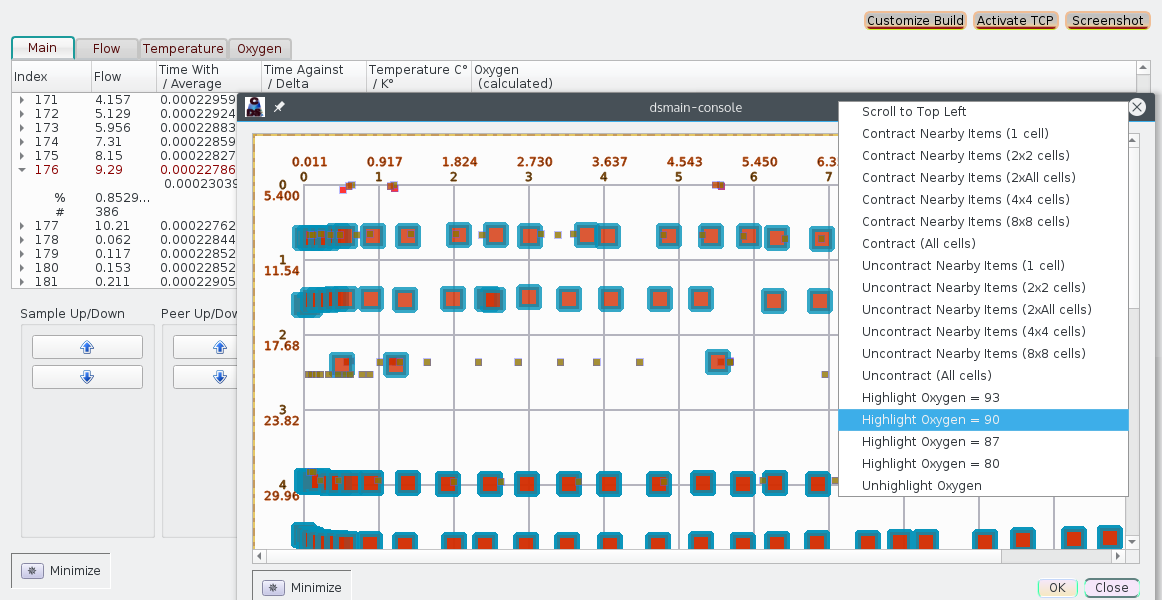
\includegraphics[width=180mm, 
    	trim={0mm 0mm 0mm 0mm},clip]
    	{pics/oxy.png}};
    
\end{tikzpicture}   
\end{figure}



\section{Multi-Application Networks in the Context of 
Scientific Research Data}
\p{Architecturally, the pattern of organization 
just described --- semi-autonomous applications 
linked together (often by virtue of being common 
extensions to an overarching \q{core} software 
platform) is 
analogous to the collection of software components 
that may share access to a data repository or 
a research-data corpus, include a corpus of 
medical/diagnostic images.  The purpose of 
research data archives --- particularly when 
they embrace contemporary open-access standards 
such as \FAIR{} (Findable, Accessible, Interoperable, 
Reusable\footnote{See \bhref{https://www.researchgate.net/publication/331775411_FAIRness_in_Biomedical_Data_Discovery}.}) 
and the Research Object 
Protocol\footnote{See \bhref{https://pages.semanticscholar.org/coronavirus-research}} --- is to promote reuse and reproduction of 
published data and findings, such that multiple subsequent research 
projects may be based on data originally published 
to accompany one book or article.  As a result, it is 
expected that numerous projects may overlap in their 
use of a common underlying data set, which potentially 
means a diversity of software components implementing 
a diversity of analytic techniques, each offering a unique 
perspective on the underlying data.  In addition to 
providing diverse analytic analytic methods, 
research-oriented software transforms the ecosystem 
where scientific data and academic books/articles 
are published and explored.  From a reader's point of 
view, open-access data sets present an interactive, 
multi-media experience which supplements reading 
article texts.  Indeed, in recent years, publishing houses 
have embraced the notion (albeit more of a future 
vision than a present reality) that conventional 
publications are only one part of a larger 
package (e.g. a \q{Research Object Bundle}), 
which may contain data, computer code, and/or 
interactive graphics alongside text-based formats 
such as \PDF{}.  At the same time, from 
a scientist's point of view, open-access research 
data offers a starting point for their own 
investigations, or a contretemps with which to 
reinforce or contrast their own findings.}

\begin{figure}

\caption{Linking Dataset Applications to Publications}
\label{fig:about}

\begin{tikzpicture}

\node[inner sep=0pt] (x1) at (0,0)
    {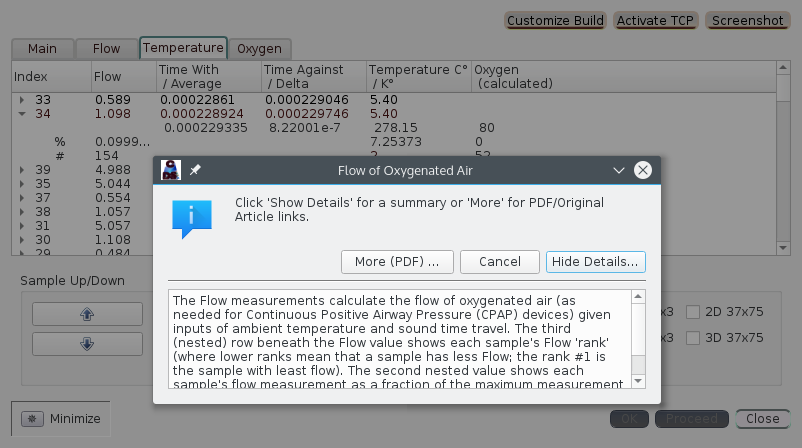
\includegraphics[width=180mm, 
    	trim={0mm 0mm 0mm 0mm},clip]
    	{pics/about.png}};

\end{tikzpicture}    
\end{figure}



\p{All of this means that scientists preparing 
academic papers are not only finalizing text 
descriptions but also, often, curating data, 
graphics, or code that demonstrates their work 
in an interactive, multi-media fashion 
(such assets are often presented to readers 
via \q{supplemental material,} \q{additional 
files,} or \q{data availability} sections 
on web pages showing article texts or abstracts).  
Scientists can support multi-media exploration 
of their research by presenting data in 
file formats used by data-visualization software; 
they can also assert more fine-grained control 
over data visualization by implementing 
custom software.  Figure~\bref{fig:oxy} illustrates 
an example of a customized data-set application 
presenting analysis in the context of 
biomedical devices (specifically, \CPAP{} 
oxygen-flow monitors) conducted by 
Dr. James A. Rodger, Professor of Management Information 
Systems and Decision Sciences at Indiana University of 
Pennsylvania (Principle Investigator 
for this project proposal).  One benefit of 
custom data-set software is the possibility 
of using \textit{microcitations} to 
connect research data (and the \GUI{} 
components where this data is visualized) 
to publication texts.\footnote{Microcitations 
are independently citeable smaller units of 
a data set, such as an individual record, 
a table column, or one table in a multi-table 
collection; see \bhref{https://www.thelancet.com/action/showPdf?pii=S1473-3099\%2820\%2930086-4}.}  
Microcitations enable application-level interoperability 
between document viewers and data-set 
applications.  For instance, individual table columns 
can be associated with specific scientific concepts 
or statistical parameters that are described 
in the article text; Figure~\bref{fig:about} shows 
an example where a user activates a context 
menu by right-clicking on a column header and 
is given a list of options, one of which yields 
to a dialog box that displays a thumbnail 
explanation of the column data and links to 
anchors in the article's \PDF{} file.  
This interop between data sets and 
\PDF{} viewers is an example of 
multi-application networking --- both the 
data-set application and the \PDF{} software 
need to be implemented or extended with 
the capacity to execute microcitation-based 
workflows.}

    \begin{frame}{\ft{Testing}}

        \begin{annotatedFigure}{0pt}{0pt}
            {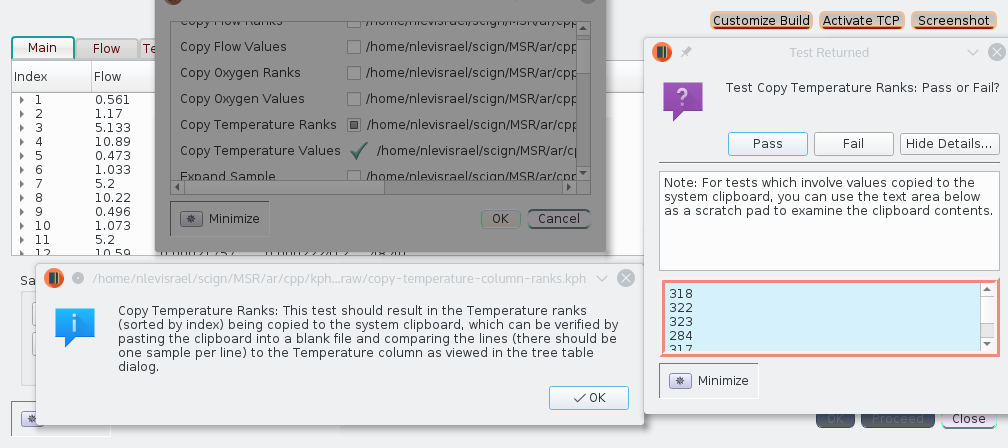
\includegraphics[scale=1]{texs/testing.png}}
            
  \node [text width=20cm,align=justify,fill=logoCyan!20, draw=logoBlue, 
  draw opacity=0.5,line width=1mm, fill opacity=0.9]
   at (0.38,0.93){\textbf{Dataset Creator includes a sophisticated 
   framework for building and running test suites to 
   ensure that raw data is processed correctly and that 
   User Interface components work properly on different 
   Operating System platforms.  This includes 
   a separate testing application that sends instructions 
   to the main Dataset Application via TCP (\circled{1}).}};

  \annotatedFigureBox{0.81,0.93}{0.903,0.982}{1}{0.903,0.935}%
  
  
   \node [text width=4cm,align=justify,fill=logoCyan!20, draw=logoBlue, 
   draw opacity=0.5,line width=1mm, fill opacity=0.9]
    at (0.08,0.64){\textbf{The testing application has several 
    features to facilitate running tests, including 
    options to repeat tests, mark success or failure (\circled{2}), and 
    examine the system clipboard (\circled{3}).}};
 
  \annotatedFigureBox{0.17,0.63}{0.37,0.685}{2}{0.37,0.63}
   \annotatedFigureBox{0.651,0.113}{0.995,0.86}{3}{0.892,0.86}% 

   \node [text width=11cm,align=justify,fill=logoCyan!20, draw=logoBlue, 
   draw opacity=0.5,line width=1mm, fill opacity=0.9]
    at (0.26,0.09){\textbf{Testers can 
    also read a description of each test (\circled{4}),  
    and view the scripts used to ceate them.}};
 
  \annotatedFigureBox{0.05,0.16}{0.62,0.325}{4}{0.62,0.19}
  
      %      \annotatedFigureBox{0.222,0.284}{0.3743,0.4934}{B}{0.3743,0.4934}%tr
      %      \annotatedFigureBox{0.555,0.784}{0.6815,0.874}{C}{0.555,0.784}%bl
      %      \annotatedFigureBox{0.557,0.322}{0.8985,0.5269}{D}{0.8985,0.5269}%tr
  
        \end{annotatedFigure}

    \end{frame}




\p{Moreover, data-set applications can provide 
(through their type system and implementation 
protocol) one form of structural model and 
formal elaboration of research theories,  
methodology, or experimental design.  
Defining an annotation schema for data sets can potentially 
be an organic outgrowth of software-development methodology 
--- viz., the engineering steps, 
such as implementing unit tests, which are essential 
to deploying a commercial-grade application.  
This point is illustrated in 
Figure~\bref{fig:testing}, which shows a \GUI{}-based testing environment for the data set depicted in Figures~\bref{fig:oxy} and 
\bref{fig:about}.  For this data set, 
the context menu actions providing column-specific functionality 
are also discrete capabilities which can be covered by 
unit tests, so the set of procedures mapped to the citeable 
concept correspond with a set of unit-test requirements.  
In this data set, these procedures are also exposed to 
scripting engines via the \Qt{} meta-object system.  In general, 
there is often a structural correlation between 
scripting, unit testing, and microcitation, so that 
an applications' scripting and testing protocol can serve 
as the basis for annotation schema and structural 
models formalizing how a data set is organized.}

\begin{figure}

\caption{Linking PDF Files with Scientific Applications}
\label{fig:il}

\begin{tikzpicture}

\node[inner sep=0pt] (x1) at (0,0)
    {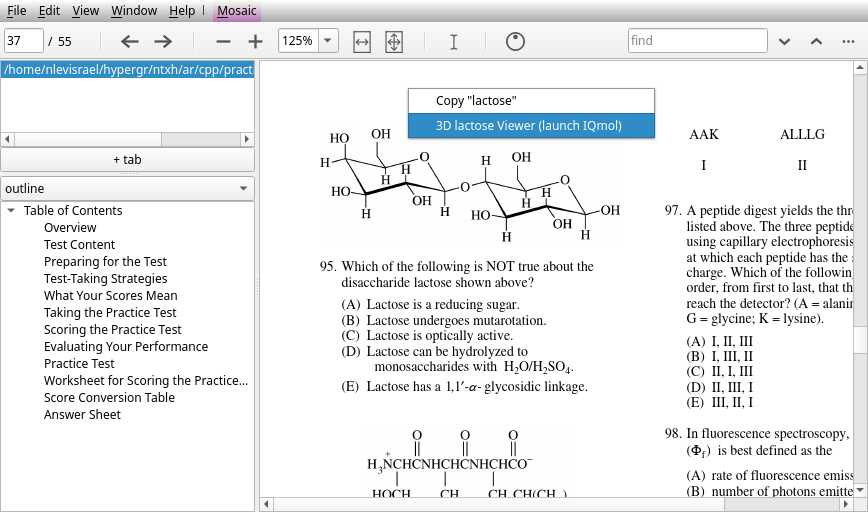
\includegraphics[width=90mm, 
    	trim={0mm 0mm 0mm 0mm},clip]
    	{pics/xl.png}};

\node[inner sep=0pt] (i1) at (10,0)
    {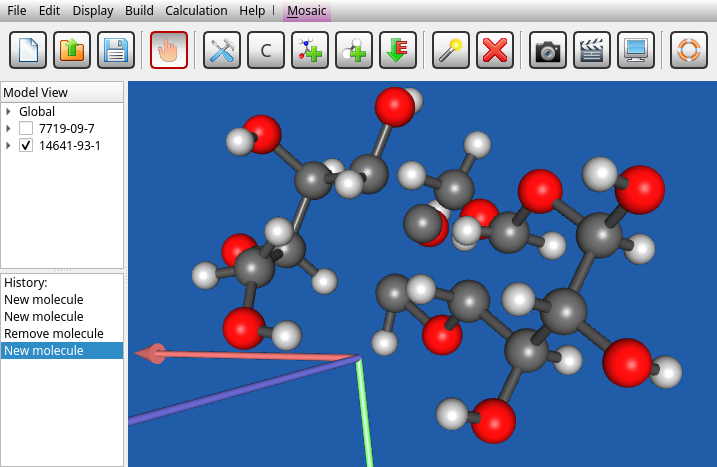
\includegraphics[width=90mm, 
    	trim={0mm 0mm 0mm 0mm},clip]
    	{pics/il.png}};
    
\end{tikzpicture}   
\end{figure}



\p{Implementing a robust research-data software 
framework involves integrating multiple scientific 
applications, but also (ideally) extending these 
applications with features specifically 
of interest to those conducting or reviewing 
research using published data sets and/or 
described in academic literature: for 
instance, capabilities to download data sets 
from open-access scientific portals; to 
parse microcitation formats; and to interoperate 
with document viewers.  Figure~\bref{fig:il} 
shows a case-study of these fearures, 
where a molecular-visualization application 
(\IQmol{}) has been extended with a multi-application 
messaging capacity allowing it to send and receive 
data from \XPDF{} (a \PDF{} viewer); in the 
figures the displayed \PDF{} document is a 
\GRE{} practice exam, and \IQmol{} is instructed 
to present a \ThreeD{} graphic visualizing the 
molecular structure of a compound 
which is the topic of a test question 
(the operation to launch \IQmol{} is provided 
as a context-menu action localized to the 
page-coordinate area close to the relevant 
question and answers on the \PDF{} viewport.
This example illustrates how applications 
within an integrated research-software environment 
can complement each other by providing 
distinct capabilities (such as interactively 
displaying Protein Data Bank files).  
A similar example is visible in Figure~\bref{fig:rad-2} 
and Figure~\bref{fig:rad-3}, which shows a multi-application 
workflow connecting \ThreeDimViewer{} 
(an example of \ThreeD{} radiology software described in the 
next section) and \MeshLab{} 
(a general-purpose \ThreeD{} visualization and 
analysis program): \ThreeDimViewer{}'s algorithms 
build a \ThreeD{} model from a \TwoD{} image series, 
and the resulting mesh file is then sent as a data 
package to \MeshLab{} so that it may be studied 
in a more fully-featured graphical environment.}

\begin{figure}

\caption{Three-Dimensional Tissue Reconstruction via 3DimViewer}
\label{fig:rad-2}

\begin{tikzpicture}

\node[inner sep=0pt] (x1) at (0,0)
    {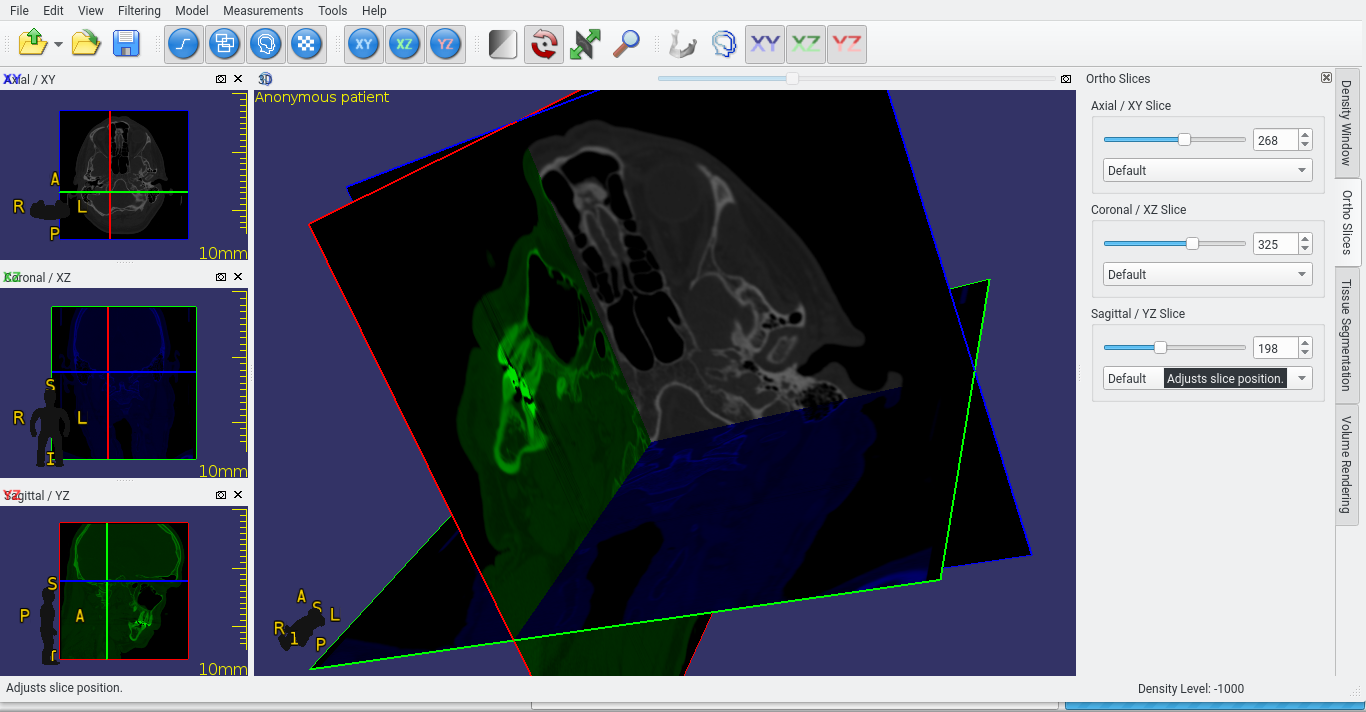
\includegraphics[width=180mm, 
    	trim={0mm 0mm 0mm 0mm},clip]
    	{pics/Rad-2.png}};
    
\end{tikzpicture}   
\end{figure}




\p{This review of data-publishing technology is 
relevant to radiology and to Patient-Centered 
Outcomes because it typifies the emerging ecosystem 
where scientific research and open-access data 
is being disseminated.  Open-access data 
publishing --- especially within the emerging 
frameworks being advocated and developed 
by publishers and research institutions 
themselves --- is conducive to a software 
engineering paradigm that favors the implementation 
of autonomous software agents which, 
their autonomy notwithstanding, can interoperate to the degree 
that they are collectively oriented to a shared data source.  
Such a multi-application network requires integration 
not only at the level of data structures, but also 
at the level of Human-Computer Interaction and 
inter-application messaging --- in the optimal 
case users can switch between applications 
based on each components' respective capabilities.  
In sum, the \CaPTk{} architecture --- consisting 
of numerous autonomous, stand-alone, native 
applications federated into a decentralized 
but unified platform --- is similar logistically 
to the kinds of application networks 
appropriate for the technology supporting 
archives of research date (including 
diagnostic-imaging repositories).}

\p{Given this architectural correlation, we propose 
that the \CaPTk{} architecture can be used 
as a prototype for implementing multi-application 
networks such as those applicable to 
research data repositories.  As a starting point 
for modeling such multi-application networks, we 
propose to concentrate on software which is 
implementationally similar to \CaPTk{} within 
the medical-imaging domain.  For example, 
\medInria{} (a general-purpose radiology 
platform) and \ThreeDimViewer{} (a tool which generates 
\ThreeD{} tissue models from \TwoD{} image series) 
are both open-source \Cpp{} applications built 
on top of the \Qt{} application development 
platform, so they occupy essentially the 
same niche in the software engineering 
ecosystem as \CaPTk{}.  Our proposed \CaPTk{}  
extensions therefore apply to these related 
projects, insofar as we can implement plugins 
extending all three applications with a more 
rigorous data-integration protocol.  Each 
of these applications likewise lends distinct 
capabilities to a multi-application radiological 
platform --- whereas \CaPTk{} is focused on 
image analysis and \AI{}, \medInria{} functions 
more as a conventional \PACS{} workstation for 
manual image-annotation and diagnostic reporting, 
while \ThreeDimViewer{} is specifically 
focused on three-dimensional tissue modeling.  
A robust data-sharing protocol 
would ensure that each of these applications can 
interoperate, allowing users the choice to 
switch which program they are using depending on 
the specific analytic tasks they wish to take on 
for a given session.}

\p{Along with these radiology-specific applications, 
the application network we are hereby describing 
can moreover include other components commonly 
used by researchers in a radiological context: 
software such as \XPDF{} (a \PDF{} viewer), 
\IQmol{} (a molecular-visualization program), 
\ParaView{} (a data-visualization platform), 
\Octave{} (an open-source Matlab alternative), 
and \Qt{} Creator (a \Cpp{} Integrated Development 
Environment) are all built with the same 
\Qt{}/\Cpp{} foundation as the three radiology 
tools mentioned above, and each of these 
applications provide capabilities sometimes needed 
for curating and conducting medical-imaging research.  
Therefore, by extending each of these applications 
with a common data-sharing and operational-integration 
protocol, we can provide scientists with a flexible 
research platform which synthesizes the capabilities 
of many popular scientific-computing applications. 
As an initial framework in which to implement this 
platform, we propose to focus on software 
tools for accessing Covid-19 research data included 
in the \RSNA{} repository, as well as other 
Covid-19 archives, such as the \Cnineteen{} 
collection of academic publications concerning 
Covid-19 and SARS-CoV-2.\footnote{See \bhref{https://pages.semanticscholar.org/coronavirus-research}.}}

\begin{figure}

\caption{The Three-Dimensional Model Exported 
from 3DimViewer to MeshLab}
\label{fig:rad-3}

\begin{tikzpicture}

\node[inner sep=0pt] (x1) at (0,0)
    {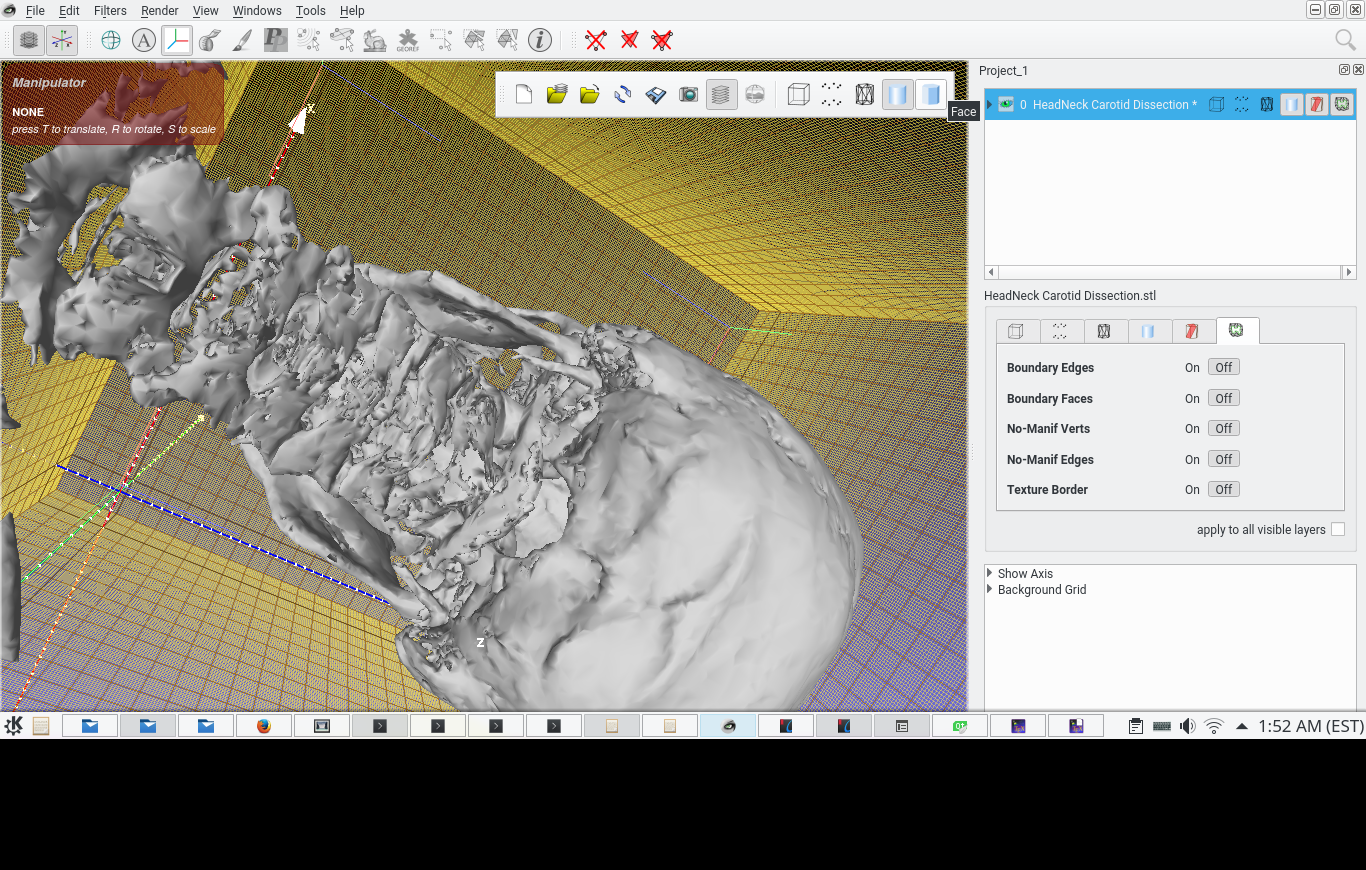
\includegraphics[width=180mm, 
    	trim={0mm 40mm 0mm 0mm},clip]
    	{pics/Rad-3.png}};
    
\end{tikzpicture}   
\end{figure}



\p{Initiatives such as Research Objects and 
\FAIR{} advocate for a technological infrastructure 
characterized by a diverse software ecosystem 
paired with a open-access research data sets.  
Scientific data repositories, linked to 
academic publishing platforms, have been engineered 
to help scientists locate and re-use data sets 
which are relevant to their research projects.  
Although formats such as Research Objects have been 
standardized over the last decade, there has not 
been a comparable level of attention given to 
formalizing how multiple software applications 
should interoperate when manipulating 
overlapping data.  The Common Workflow Language 
(\CWL{}), which has been explicitly included in the 
Research Object 
model\footnote{see \bhref{http://www.researchobject.org/scopes/}},
documents one layer of inter-application messaging, 
including the encoding of parameters via command-line 
arguments; \CaPTk{} provides a \Cpp{} implementation of 
\CWL{} and uses it to pass initial data between 
modules.  Serializing larger-scale data structures 
is of course a generic task of canonical encoding 
formats such as \JSON{}, \XML{}, \RDF{}, and 
Protocol Buffers --- not to mention text or binary 
resources serialized directly from runtime objects 
via, for instance, QTextStream and QDataStream.  
This means that some level of inter-application 
communications is enabled via \CWL{}, and 
that essentially any computationally tractable 
data structure can be encoded via formats such 
as \XML{}.  These solutions, however, are 
sub-optimal: \XML{} (as well as \JSON{} and analogous 
formats) is limited because it takes additional 
development effort to compose the code that marshals 
data between runtime and serial formats.  
Similarly, although \CWL{} can model information 
passed between applications, it provides 
only an indirect guide to programmers implementing 
each applications \q{operational semantics} --- 
viz., the procedures which must be executed 
before and after the event wherein data is 
actually passed between endpoints.}

\p{In the context of \CaPTk{}, for example, 
integrating peer modules with the \CaPTk{} core 
application involves more than simply 
ensuring that these endpoints communicate 
via a standardized data-serialization format: 
the plugins must be \textit{registered} 
with the core application, which affects the 
core in several areas, including the build/compile 
process and construction of the main \GUI{} 
window.  Modeling the interconnections between 
semi-autonomous modules, as \CaPTk{} demonstrates, 
therefore require more detail than simply 
modeling their shared data encodings; it 
is furthermore necessary to represent all 
procedural and User Interface requirements 
in each component that may be affected by 
the others.  Despite the standardization 
efforts that have been invested in 
Research Objects and the Common Workflow Language, 
we contend that this fully detailed 
protocol for multi-application interop has not 
yet been rigorously formalized.  As part of 
our project for extending \CaPTk{} and then 
generalizing this extension to scientific 
research platforms (not necessarily restricted 
to radiology), we propose to ameliorate 
this situation by implementing a more rigorous 
protocol for multi-application networking, 
which we will call the 
\q{Hypergraph Multi-Application Configuration Language} 
(\HMCL{}).  This language is paired with a new 
data-exchange protocol that we are also implementing, 
the Hypergraph Exchange Format (\HGXF{}), 
both of which are summarized in the next section.}

\section{Our proposed Hypergraph Exchange Format and 
Hypergraph Multi-Application Configuration Language}
\p{To explain the rationale for \HMCL{} and \HGXF{}, 
consider the role that data-serialization and Interface 
Definition languages play in software engineering: 
programmers need guidelines when implementing 
procedures wherein one application sends, receives, 
and/or acts upon data sent or requested by a 
second application.  Standardized representation 
formats provide specifications that help codewriters 
serialize data in ways that produce usable resources 
--- representing data via \XML{}, for instance, ensures 
that any application has the theoretical capacity 
to decode the information (insofar as \XML{} libraries 
exist for every mainstream programming language 
and environment).  Optimally, both end-points in a 
cross-application messaging scenario should be 
able to encode and decode information with 
as little \q{biolerplate} code as possible, which 
is why applications may choose serialization 
languages which are detailed and expressive, 
so long as they have guarantees that partner 
applications can recognize the same format.  
This is one justification for hypergraph 
serialization, insofar as hypergraphs are 
a very flexible representation that can 
accommodate almost any data structure 
that needs to be encoded, often with 
less translational effort than marshaling 
data into formats such as \XML{} and \JSON{}.}

\p{Hypergraphs provide a generalization of 
graph-like and/or hierarchical data structures 
in multiple contexts: in markup languages, 
for example, hypergraphs allow for concurrent 
or overlapping node-structures, yielding 
formats which are more expressive than \XML{}.  
In the Semantic Web, hypergraphs are used 
as a generalization of \RDF{}, allowing for 
nested levels of structure and for data localization.  
Within image analysis, hypergraphs are often 
employed to represent feature vectors and/or 
geometric relations between image segments.  
Hypergraphs have also been utilized in the
description of multi-part biological or 
biomedical processes: protein complexes, 
metabolic reactions, genomic sequences, 
and so forth.  Considering the range of 
specialized cases for hypergraph representations 
--- as well as how hypergraph structures are 
suitable for simpler data that could also 
be represented via \XML{} or \RDF{} --- 
it is reasonable to select hypergraphs 
as a generic data-encoding format.  
We propose a flexible hypergraph model which 
can accommodate various hypergraph 
categories (e.g., both directed and 
undirected) and can represent supplemental 
information sometimes introduced into 
hypergraph models, such as probabilities 
(inserting measures of uncertainty or 
fuzziness into relations) and \q{roles} 
(characterizing multi-part relations in terms 
of the situational status of their 
constituents).\footnote{The concept of roles 
is highlighted by Grakn.ai: see \bhref{https://dev.grakn.ai/docs/schema/concepts}.}  The general category of hypergraphs encompasses a 
range of structures implemented by various 
hypergraph libraries and database engines.  Although 
several graph-serialization formats currently 
exist, we believe a new Hypergraph Exhange Format 
is warranted which is intrinsically designed 
to model the full range of hypergraph structures 
developed in the scientific literature as well 
as the scientific-computing community.}

\p{This discussion illustrates the rationale for 
designing our \HGXF{} format.  As mentioned above, 
this format is intended to be paired with a Hypergraph 
Multi-Application Configuration Language 
(\HMCL{}).  The purpose of \HMCL{} is to represent 
multi-application networking protocols with greater 
procedural detail and specificity than provided 
by traditional workflow or Interface Definition 
languages.  Within the scope of multi-application 
workflows, we have, in prior paragraphs, briefly outlined 
the protocols adopted by \CaPTk{}.  A more rigorous 
review of multi-application networking can be obtained 
by considering analogous protocols connecting 
semi-autonomous software agents in other contexts: 
\ParaView{} extensions, \Qt{} Creator Plugins, \Octave{} 
scripts, and \ROOT{} modules, for example 
(\ROOT{} referring to the physics platform developed 
at \CERN{}) --- restricting attention to the 
\Qt{}/\Cpp{} ecosystem.  Further afield, a similar 
sense of semi-autonomy can be found in hybrid \GUI{} 
and scripting platforms such as Jupyter (in the 
Python context) and Seco (a Java-based \q{notebook} 
framework built on top of HyperGraphDB, where 
\textit{notebook} in this environment refers to 
interactive code development and execution 
containers such as Jupyter and RStudio).  
These platforms are familiar to data visualization 
and machine-learning engineering (where a script 
may analyze data and a \GUI{} component follow up 
by presenting a chart or dataplot summarizing the 
analysis), as well as other quantitative 
domains outside the natural scientists 
(in financial services, for example, scripting 
formats such as \MQFour{} execute investment strategies 
while associated \GUI{} components present 
finance-related visual objects, such as candlestick charts.)  
Similar workflow models have been developed in 
theoretically-informed frameworks such as 
\VISSION{}, which is paired with programming constructs 
such as \q{metaclasses} and \q{dataflow 
interfaces}.\footnote{See \bhref{https://pdfs.semanticscholar.org/1ad7/c459dc4f89f87719af1d7a6f30e6f58dff17.pdf}; note that 
this is a different project than the ViSion Ontology 
referenced earlier.}     
The common element in all of these systems is the 
presence of a central \GUI{} application whose 
capabilities are enhanced by customizable extensions with 
their own analytic and/or \GUI{} features: these 
extensions are neither fully autonomous 
applications nor simple scripts that may automate 
certain capabilities of the main application but 
do not fundamentally extend its functionality.  
This intermediate position --- neither wholly 
autonomous nor functionally subservient --- 
is expressed by the idea of \textit{semi-autonomous} 
software agents.}


\p{Rigorous models of application networks among semi-autonomous 
components acquire an extra level of complexity precisely 
because of this intermediate status: protocol definitions 
have to specify both the functional interdependence 
and the operational autonomy of different parts of 
the application network.  We propose to 
address this complexity by adopting a hypergraph-based 
paradigm for procedural and type modeling, from 
which derives our proposed \HMCL{} 
format.\footnote{A preliminary characterization 
of hypergraph-based type systems (and their 
corresponding representation of detailed 
procedural signatures and requirements) 
can be found in Nathaniel Christen's chapter 
(chapter 3) in \textit{Advances in Ubiquitous Computing: 
Cyber-Physical Systems, Smart Cities and Ecological Monitoring}, 
edited by Dr. Neustein 
(see \bhref{https://www.elsevier.com/books/advances-in-ubiquitous-computing/neustein/978-0-12-816801-1}).} 
The goal of \HMCL{} is to define protocols for 
inter-application messaging by focusing on 
procedures enacted by both applications before and 
after each stage in the communication.  This 
is not (in general) a \q{Remote Method Invocation} 
or \q{Simple Object Access Protocol} where one 
application explicitly initiates a specific procedure 
for the second to perform; instead, the chain of 
procedure calls (which we call the multi-application
\textit{operational semantics}) is more indirect, 
with \textit{requests} and \textit{responses} that 
may be mapped to different procedure-sequences in 
different contexts.  Nevertheless, although 
one application does not need detailed 
knowledge of the other's internal procedure 
signatures (which would break encapsulation), 
a rigorous messaging protocol can be developed 
by specifying requirements on the relevant 
procedures implemented by each application.  
Developers can then explicitly state that 
a given set of procedures implements a given 
\HMCL{} protocol (the multi-application documentation 
thereby has more detailed information about 
application-specific procedures than each 
application has \visavis{} its peers).  The 
functional interdependence between applications can 
accordingly be modeled by defining protocols which 
must be satisfied by procedure-sets internal 
to each end-point --- the relevant information 
from an integrative standpoint is not the 
actual procedures involved, but confirmation 
that the relevant procedure sets adhere 
to the relevant multi-procedural protocol.}

\p{Reviewing the source code and documentation 
for \CaPTk{} confirms that multi-application 
messaging along these lines is implicitly adopted 
by \CaPTk{}, but the protocols involved have not 
been formalized with the level of rigor we 
contend is possible via \HMCL{}.  As the 
central element in our extension to \CaPTk{}, 
we propose therefore to formalize the \CaPTk{} 
protocol using \HMCL{}, which among other 
benefits will allow plugins to be introduced 
into \CaPTk{} via configuration files rather than 
through the manual process described in the 
\CaPTk{} literature.\footnote{See for example 
\bhref{https://www.med.upenn.edu/cbica/assets/user-content/images/captk/2018_ISBI_CaPTk.0404.Part2.pdf}, particularly 
the material starting on the 30th slide of that presentation.}  
At a practical level, we believe these enhancements to 
\CaPTk{} will make it a little easier for \CaPTk{} to be 
used in a context where researchers wish to 
analyze clinical outcomes in conjunction with 
image data within the scope of statistical, 
Machine Learning, or \AI{} methods.  Moreover, 
they will allow \CaPTk{} to be integrated with 
other radiological software (such as \medInria{} and 
\ThreeDimViewer{}) and, more generally, with a 
suite of scientific applications, arriving at a 
multi-purpose research platform optimized for the 
curation and re-use of open-access research data.  
At a more theoretical level, we also believe 
that the formats we have described here --- specifically 
\HGXF{} and \HMCL{} --- can be useful in a wide 
range of scientific computing and software engineering 
contexts, particularly in conjunction with 
\q{reference implementations} that we will provide 
in the context of \CaPTk{}.} 

\section{Hypergraph Ontologies, and a Concrete Hypergraph Ontology for Radiological Outcomes} 
\p{As explained above, the goal of \HGXF{} is to  
provide a general-purpose hypergraph representation 
format, suitable for all hypergraph data structures 
as well as any structures which are categorically subsumed 
by hypergraphs (such as \RDF{} graphs).  
Consequently, \HGXF{} is designed in part by 
examining existing Hypergraph Database software 
(such as HyperGraphDB, AllegroGraph, and Graken.ai)  
and runtime hypergraph libraries, as well as 
academic literature where hypergraph analyses have 
been used for (e.g.) image-segmentation and 
Machine Learning algorithms.  These resources 
provide an overview of the range of data structures 
which need to be encoded by a general-purpose language 
such as \HGXF{}.  The design of \HGXF{} has also 
been influenced by the Semantic Web, insofar as 
hypergraphs are a generalization of the directed, labeled 
graphs that are the building-blocks of the Semantic Web.  
At the same time, hypergraphs --- along with 
structures that can be modeled via hypergraphs, 
such as Conceptual Spaces --- are an improvement 
on Semantic Web data formats and schema, addressing 
the limitations of a paradigm devoted to modeling 
complex information via first-order logic and 
non-nested graphs, with no notion of scoping or 
locality.\footnote{These are familiar critiques, but 
laid out with particular thoroughness by the 
Conceptual Space community: see \bhref{http://idwebhost-202-147.ethz.ch/Publications/RefConferences/ICSC_2009_AdamsRaubal_Camera-FINAL.pdf} 
and \bhref{https://pdfs.semanticscholar.org/1d58/faa5cb23efb7394aeb3dfe688edd99797a91.pdf}.} }


\p{At the same time, a lot of effort has been extended 
building technologies to integrate heterogeneous 
data spaces via the Resource Description Framework 
(\RDF{}) and \RDF{} ontologies; it would be irresponsible 
to ignore these contributions.  In radiology, for 
example, attempts to better incorporate clinical 
and outcomes data are centered on ontologies such 
as \RadLex{}, \ViSion{}, and \SeDI{}; insofar 
as these are (or have potential to become) 
canonical reporting standards, Patient-Centered 
research should promote rather than critique 
these initiatives.  As a result, the important 
consideration is how to employ hypergraphs as an extension 
to the Semantic Web when warranted while preserving 
the virtues (and interoperating with) 
conventional \RDF{} ontologies.}

\p{The idea that hypergraphs \textit{extend} 
but do not \textit{replace} \RDF{} and the 
Semantic Web implies that hypergraph schema 
are extensions of (but not substitutes for) 
\RDF{} ontologies --- which in turn 
yields the notion of \textit{hypergraph 
ontologies}.  In a conventional \RDF{} ontology, metadata is primarily 
associated with graph nodes and edges.  In particular, 
nodes are referenced to Uniform Reference Identifiers 
(\URI{}s), such as web addresses, and edges are labeled 
with concepts formally defined in one or more ontologies.  
Concepts which are used to annotate graph-edges, and which are 
given a fixed meaning in some controlled vocabulary, are 
often called \q{properties.}  One special \q{is-a} property 
is often used to connect nodes with concepts that 
classify entities into one of many categories defined 
in an ontology, often called \q{classes.}  As such, most 
\RDF{} ontologies are primarily composed of 
\textit{classes} and \textit{properties}, each assigned 
a unique label.  The purpose of metadata for a given graph 
is then to link nodes to classes (for example, specifying 
that one node represents a clinical trial and the second 
represents a patient), and furthermore link edges to properties 
(for example, specifying that a patient-node is connected 
to a trial-node in that the patient is \textit{enrolled in} 
the trial).}

\p{Hypergraph ontologies are similar to conventional 
\RDF{} ontologies in that they likewise provide 
constraints and metadata for graphs.  However, 
hypergraph ontologies are more complex because hypergraphs 
are likewise more complex than ordinary graphs.  In particular, 
hypergraphs have different layers of structure:  
whereas \RDF{} nodes are intended to represent a 
single concept or value (such as a number, date, 
personal name, or \URL{}), a \textit{hypernode}, within a 
graph, typically encompasses multiple pieces 
of information inside it (often called \textit{hyponodes}, 
\textit{projections}, \textit{inner elements}, 
\textit{roles}, or just \textit{nodes}).
\footnote{%
The term \q{roles} is used by Grakn.ai 
(see \dhref{https://dev.grakn.ai/docs/schema/concepts}); 
\q{projections} is used by HyperGraphDB (see 
\dhref{http://www.hypergraphdb.org/?project=hypergraphdb&page=RefCustomTypes}); 
\q{inner entity} is used by the biointelligence project 
(see \dhref{https://www.ncbi.nlm.nih.gov/pmc/articles/PMC3555311/}), 
where the corresponding notion of \q{external entity} 
refers to what in other contexts might be called 
other hypernodes linked to a given hypernode via hyperedges.}  
In general, when analyzing hypergraphs it is necessary to 
distinguish at least two \q{tiers} of nodes, 
\textit{hypernodes} and \textit{hyponodes}, such that 
hyponodes are contained within hypernodes.  As a result, 
hypergraph ontologies need a corresponding distinction 
for node and edge annotations: insofar as nodes are 
categorized via classes, and edges via properties, 
it is necessary to stipulate whether these classifications 
apply to hypernodes, hyponodes, or some combination of the two.}

\p{A further complication (contributing to the complexity of hypergraph 
ontologies compared to \RDF{} ontologies) arises because, 
even though hypergraphs represent nested or hierarchical structures,  
these hierarchies are often partial or overlapping. 
For example, a patient is \textit{part of} a 
clinical trial, but a patient is also included in 
other collections as well; for instance, a patient 
may be enrolled in a specific health plan 
(for insurance coverage).  One technique for modeling 
overlapping hierarchical data via hypergraphs is to 
employ \q{proxies,} which are digital identifiers encoding a 
multi-faceted concept into a single value that can be 
part of a hypernode (proxies are similar to 
\q{foreign keys} in \SQL{}).  Therefore, each patient, represented 
by its own hypernode, has an identifier which can be a 
proxy-value for the patient; for example, a value 
assigned to a hyponode becomes included 
in the hypernode encoding the list of patients enrolled 
in a clinical trial, or in the hypernode 
encoding the list of patients enrolled 
in a specific health plan.  Hypernodes can then be linked to 
other hypernodes by virtue of proxies (e.g., the 
trial-to-patient connection), and also by 
virtue of overlap (e.g., the set of all patients 
both enrolled in a given clinical trial \textit{and} 
enrolled in a given health plan).}

\p{In sum, compared to \RDF{} --- where there is one 
single sort of node-to-node relationship, based on 
whether or not an edge exists betweel nodes and 
how this edge is labeled --- hypergraphs are more 
flexible/expressive because they have 
multiple genres of node-to-node relationships: 
the relation between hypernodes and their inner 
hyponodes; between hypernodes and one another; 
between hyponodes in different hypernodes; 
and variations on each of these relation-types 
wherein relations are defined indirectly through 
proxies.  Moreover, in addition to hypernodes 
and hyponodes, hypergraphs afford additional 
levels of detail, such as \textit{frames}, 
\textit{channels}, and \textit{axiations}.
All of these details provide different 
\q{sites} where hypergraph annotations and 
metadata may be defined.\footnote{This means that 
formats for describing hypergraph ontologies 
have to be more expressive than \RDF{} ontologies, 
because \RDF{} ontologies need only to classify 
metadata as node-annotations or edge-annotations; 
by contrast, hypergraph ontologies need to distribute 
annotations among multiple sites of graph structure.}}

\p{An additional distinction within the Semantic Web 
is the contrast between \textit{reference ontologies} and 
\textit{application ontologies}.  In general, \textit{reference 
ontologies} are general-purpose schema intended to 
establish conventions shared by many different applications, 
to ensure that a large collection of data-producing software 
in a given domain is interoperable.  By contrast, 
\textit{application ontologies} are narrower in scope 
because they are more tightly integrated into applications that 
directly send and receive data.  Ontologies 
of either variety are used by software to interoperate 
with other software: so long as two applications are 
using the same ontologies, it is possible to 
ensure that one application can understand the 
data produced by a second, and vice-versa.  
However, such inter-operability is only potential; 
it is the responsibility of programmers to 
actually implement code which produces and/or 
consumes data that conforms to the relevant 
ontology specifications.  In general, application 
ontologies are structured in such a way that 
these concrete implementations are more straightforward 
to produce, compared with reference ontologies.  
Reference ontologies offer little guidance to 
developers \visavis{} how to directly support the 
ontology within application code.  Conversely, 
application ontologies more rigorously describe the 
data structures which applications must implement 
in order to properly manipulate data that is structured 
according to the specifications of the ontology.}

\p{Within data mining and image analysis, hypergraph 
models are used in different ways for different 
algorithms.  In the context of Covid-19 radiology, 
\bhref{https://arxiv.org/pdf/2005.04043.pdf} 
describes an algorithm for assessing the probability 
of SARS-CoV-2 infection from chest \CT{} scans, 
where hypernodes represent high-dimensional 
vectors (191 dimensions overall) and hyperedges 
represent k-nearest-neighbors; here each hypernode 
represents an entire image, mapped to a 191-dimensional 
feature-vector.  In contrast, other image-analysis 
methods use hypernodes to designate smaller segments 
\textit{within} the image, where hyperedges 
designate geometric adjacency and/or feature-space 
similarities.  Whatever the algorithm, hypergraph 
analyses would employ a hypergraph library 
to store preliminary data for analysis and/or for 
serialization within a data set.  One benefit of a 
Hypergraph Application Ontology is therefore that 
these data structures used internally to implement 
analytic methods can be directly expressed within 
the ontology, whereas \RDF{} ontologies can only 
model hypergraphs indirectly.}

\p{Although it is theoretically possible to encode 
data directly via \RDF{} graphs, it is far more 
common for applications to employ tabular and/or 
hierarchical formats such as spreadsheets, Protocol Buffers,
\XML{}, or \JSON{}.  As a result, the role of ontologies 
for constraining data structures (so that they adhere 
to common standards) is indirect.  It is useful to 
remember that ontologies are, at their most basic level, 
Controlled Vocabularies; as such, ontology constraints often 
amount to stipulating a set of acceptable terms for a data 
value, column header, or annotation.  For a trivial example, 
our calendar recognizes 12 month names and 7 day names, 
which constrain the set of values permissible for \q{month} 
and \q{day} within a calendar date.  These terms are 
so commonplace that a \q{date ontology} is unnecessary, 
but in scientific or technical domains it becomes 
necessary to define vocabularies of allowable 
names or labels for specific data fields that 
representing some scientific value or measurement.  For instance, 
the Ontology of Vaccine Adverse Events (see 
\bhref{https://jbiomedsem.biomedcentral.com/articles/10.1186/2041-1480-4-40}) provides a nomenclature for use in Adverse Events Reporting, 
so that researchers or clinicians can describe symptoms via canonically 
recognized terms rather than through informal 
text descriptions.  In general, ontologies constrain 
data sets by stipulating that particular individual 
values within the overall data collection have names or descriptions 
whose associated set of possible values is prescribed \textit{a priori} 
by the applicable ontology.  However, the relationship between 
ontologies and concrete data sets must itself be 
documented, which is where application ontologies 
can become relevant --- application ontologies provide 
a bridge between reference ontologies and the 
applications which use them (along with the data 
generated and shared by those applications).}

\p{In order to preserve the benefits of \RDF{} 
ontologies --- while also addressing those lacunae 
which make the Semantic Web \q{not (really) semantic} 
--- hypergraph ontologies need to model constraint 
schema on hypergraph constructions (which have 
significantly more parameters of structuration 
than \RDF{} graphs) while also connecting 
these schemas to the Controlled Vocabularies 
and logical axioms of Semantic Web (particularly 
\OWL{}) ontologies.  There are as such 
several areas of detail within hypergraphs 
where links to \RDF{} ontologies may be 
drawn, which are outlined here:\footnote{A 
full explanation of these concepts and terminology 
depends on an in-depth treatment of hypergraph 
type theory, which is outside the scope of 
this proposal.}

\begin{description}

\item[Hypernodes' Cocyclic Type Structure]
One of the central principles of hypergraph data modeling 
is the use of \textit{hypernode types} to 
specify what sort of information is necessarily 
associated with a hypernode.  In particular, 
a hypernode encompasses multiple hyponodes, 
each with their own type.  These hyponodes 
represent information in some sense 
\q{contained within} or \q{tightly connected  
to} a hypernode (whereas data less canonically 
associated with each hypernode would, in 
general, be asserted via hyperedges rather than 
via hypernode/hyponode containment.  In order 
to ensure that hypergraphs are predictably 
organized, hypernodes cannot have arbitrary 
collections of hyponodes, but must instead 
be aggregates of hyponodes which are assembled 
according to a schematic pattern, defined in 
terms of hyponode types.  For maximum generality, 
a hypergraph type system should allow hyponode-type 
patterns to be as flexible as possible without 
introducing a need for metadata asserted at the 
level of individual hypernodes rather than hypernode 
types; this motivates the idea of a \q{cocyclic} 
type system which is minimally constrained 
(but not unconstrained).\footnote{A pattern 
of hyponode types can be called \q{cocyclic} 
if the type-sequence includes a (possibly empty) 
tuple of types with no requisite pattern 
(called the \q{precycle}) followed by a 
repeatable type-tuple.  Cocyclically typed 
hypernodes therefore represent expandable 
data structures such as lists, stacks, 
queues, deques, and dictionaries.  A typical 
hypernode type may indirectly include multiple 
collections-types via proxies.}   
When translating \RDF{} ontologies to hypergraph 
schema, then, one consideration is whether 
edge-requirements are sufficiently ubiquitous 
in some context (e.g. with respect to some 
\textbf{rdf:class}) that these edges should 
be translated to hypernode/hyponode inclusions, 
and then to define a pattern of hyponode types 
for the corresponding hypernode type.

\item[Roles, Projections, and Dimensional Annotations]
A hypernode type provides a schema defining a 
sequence of hyponode types; it is sometimes 
said that the hypernode \q{projects onto} that 
space of hyponode types.  This projection is 
minimally characterized by hyponode types, 
but some hypergraph systems allow the 
projection to be \textit{annotated}, introducing 
additional metadata that constrain 
(or augment the expressive power of) the 
enclosing hypergraph.  Annotations can 
define scales/units/levels of measurement, 
probability distributions, situational roles, 
and other details lending semantic grounding 
to the data-field encapsulated by a hyponode.  
This metadata can then be a vehicle for 
translating \RDF{} class constraints to 
hypergraph schema. 

\item[Semantic Nominal Dimensions]
The most direct translation of 
Controlled Vocabularies to a hypergraph context 
is often that of constraining the space 
of variation for one specific project to 
a set of allowable terms.  In the typical 
case, a hyponode type encapsulates a 
nominal set of values (i.e., an enumeration), 
so any hypernode including that type as one 
of its projects is constrained by the 
labels registered in the vocabulary 
(a related formulation replaces 
non-hierarchical vocabularies with 
\textit{taxonomies}, where some labels 
are treated as more or less granular 
variants of others).

\item[Dimension Aggregates, Domains, and Conceptual Spaces]
Conceptual Space Theory --- which has been applied 
toward the analysis of data structures and 
cognitive patterns in science, linguistics, 
and \AI{} --- can be modeled in the 
hypergraph context by noting that hyponode 
projections are sometimes interdependent: 
dimensions tend to aggregate into semantically 
related groups (like \textit{latitude} and 
\textit{longitude} as geographic markers).  
In Conceptual Space models, accordingly, 
projections are split into two 
levels --- \textit{dimensions} and 
\textit{domains} --- while other 
dimensional-analytic constructions 
(such as scales and units of measurement) are 
carried over.\footnote{See \bhref{https://pdfs.semanticscholar.org/521a/cbab9658df27acd9f40bba2b9445f75d681c.pdf}, 
\bhref{https://arxiv.org/pdf/1703.08314.pdf}, 
or \bhref{http://lup.lub.lu.se/record/1775234}.}  
Conceptual Space Theory also then introduces 
concepts of fuzzy logic or \q{convexivity} 
(according to different metrics) to simulate 
patterns in human 
conceptualization.\footnote{A good review is 
provided by the publications and code archived 
at \bhref{https://github.com/lbechberger/ConceptualSpaces}.}
  
\item[Probabilistic, Temporal, and Overlapping Hypergraphs]
Other forms of metadata constrained via ontologies 
can be expressed in terms of annotations 
defining weights or probabilities on 
hypernodes and/or hyperedges.  One example is 
the juxtaposition of alternative markup hierarchies, 
in the context of hypergraph representations for 
Concurrent Markup languages such as \TAGML{}.  
Numeric edge-annotation can represent 
weights (e.g., provide measures of the degree 
of uncertainty in the edge's relation actually 
obtaining), but constructions similar to 
weights have other sorts of applications.  
For instance, edge-annotations can be measures 
of time-spans, allowing hypergraphs to 
describe \q{entity-event models.}\footnote{See 
\bhref{https://allegrograph.com/consulting/entity-event-knowledge-graphs/}.}  These models are particularly inportant 
for patient-centered data via their use in 
analyzing clinical outcomes by aggregating data 
according to patient-centered reviews 
extracted from \EHR{} 
data.\footnote{See \bhref{http://exploreclg.montefiore.org/upload/training-materials/The\%20Cohort\%20ParadigmV30.pdf}.}
  
\item[Proxies, Inverted Proxies, and Double-Inverted-Proxy Constructions]
As described earlier, hypernodes can assert \q{containment} of 
other hypernodes by containing a \textit{hyponode} which 
\textit{proxies} the second hypernode.  
An \textit{inverted proxy} connection is therefore 
the mirror-image of this assertion 
(which may or may not be formally recognized 
by the hypergraph).  A \textit{double-inverted-proxy} 
connection is accordingly the relation obtaining 
between two hypernodes which are both proxied by 
one third hypernode (using the earlier example 
of proxies, the fact that two patients 
are enrolled in the same clinical trial).  
Many graph connections identified in a 
Semantic Web context (e.g., by \SPARQL{} queries) 
are likely to translated to double-inverted proxies 
in a hypergraph context.  
\end{description}

In general, these hypergraph constructions represent 
sites for asserting constraints that 
(for \RDF{} ontologies) would be defined on 
classes or properties; they are therefore 
a natural scaffolding for translating \RDF{} ontologies 
to hypergraphs.  Such a translation 
mechanism allows existing ontologies 
--- which may play a valuable role 
in specifying protocols for workflows 
and data-sharing between software components  
--- to be reused in a hypergraph modeling environment.}

\p{As illustrated by \CaPTk{}, multi-application workflows 
are characterized both by the data which is 
transferred between applications and by the 
operations which connect the two applications 
--- that is, the procedures enacted by 
each application when they become operationally 
linked.  As a preliminary model, we can identify 
two stages of operational connection between 
an already-running application (which may be 
called the \textit{primary} component) 
and a second application launched by the primary 
(which may be called the \textit{peer} component).  
The first stage occurs when the primary component 
launches the peer component, and is characterized 
by two operational sequences: procedures enacted 
by the primary prior to this launch, and procedures 
enacted by the peer subsequent to the launch.  
A second stage occurs when the peer component 
has completed its actions, and sends data back 
to the primary component, which again involves two 
operational sequences: procedures enacted by the 
peer prior to the transfer, and procedures enacted by the 
primary subsequent to the transfer.  Fully describing 
the procedural workflow therefore entails specifying 
four operational sequences: primary, then peer, 
during the launch stage; and peer, then primary, 
during the transfer stage.  A schema describing 
the operations performed during these four sequences 
can be called a \textit{procedural ontology}.}

\p{Consequently, rigorous models of multi-application networks 
should \textit{synthesize} information about data structures 
(the type of information shared between application-points) 
with information about procedural workflows 
(describing operational sequences prior to 
the launch and transfer stages of a multi-application linkage).  
The synthesis of this structural and procedural information 
can be called a \textit{procedural application ontology}.  
Insofar as the new \HMCL{} language defines the operational 
semantics of multi-application workflows, \HMCL{} 
can be seen as a format for asserting and 
integrating procedural application ontologies (according 
to this definition).}

\p{Insofar as \PACS{} and \DICOM{} systems need 
to be paired with applications in the other 
categories (such as image and data-set analysis), it is 
important to develop radiological Application Ontologies, 
alongside the canonical Reference Ontologies 
associated with diagnostic imaging.  As such, starting with 
the Covid-19 context, but designed for more 
general applications as well, our proposal includes 
the development of a novel radiology-focused \textit{application} 
ontology, specifically the \q{Hypergraph Ontology 
for Diagnostic Imaging, Clinical 
Outcomes, and Data Mining} (\HDICOM{}).  The goal 
of \HDICOM{} is to connect \RDF{}-based 
radiological ontologies with software applications 
designed to manipulate radiological (and corresponding 
treatment and outcomes) data.  
In addition, \HDICOM{} will formalize 
the data-sharing protocols implicitly adopted 
by software aggregates such as \CaPTk{} 
(this part of the ontology will be expressed 
via \HMCL{}).} 


%\p{}

%\p{}

%\p{}



\section{Conclusion}
\p{In sum, then, the following represents 
contributions that we propose for inclusion into 
patient-centered outcomes research in the 
Covid-19 context, as prioritized by the 
current funding opportunity: first, we 
will implement an extended radiological 
software platform which both utilizes and 
improves upon the extension mechanism present 
in \CaPTk{}, and then integrates other radiological 
software as well, such as \medInria{}.  
We will develop extensions that allow researchers 
to cross-reference radiological and clinical/outcomes 
data, by introducing more sophisticated 
data models and protocols for sharing patient-centered 
information among points in a multi-application network, 
such as those present between \CaPTk{} and its 
extensions, or (given our expanded platform) between 
\CaPTk{} and other radiological applications, 
such as \medInria{}.  Second, we will implement a 
multi-faceted research platform oriented toward 
open-access scientific data sets, particularly 
the \AI{} Image Repository for Covid-19 currently 
being curated by \RSNA{} (and scheduled to be 
published within the time-frame of this project-proposal).  
Third, we will formalize and provide reference implementations 
for a new data serialization format (\HGXF{}) and a new 
interface and workflow description language (\HMCL{}) 
which are applicable to a wide range of scientific 
domains; we will ensure that these languages are 
particularly optimized for representing patient-outcomes 
data and for configuring inter-application messaging in 
contexts where special protocols have to be observed 
so as to curate medical information in ways that 
prioritize patient-centered outcomes.  To 
concretely link radiological and outcomes data, 
we will formalize the \HDICOM{} ontology as one 
schema constructed via \HGXF{} and \HMCL{}.}

\p{The implementations hereby proposed as contributions to 
the PCORnet initiatives coincide with software being 
developed for the forthcoming Elsevier 
volume (mentioned in the Introduction) 
titled \textit{Cross-Disciplinary Data 
Integration and Conceptual Space Models for Covid-19}, 
co-authored by Amy Neustein and Nathaniel Christen.   
Dr. Neustein is the Administrative Officer for 
this proposal and Nathaniel Christen is the developer 
who has implemented prototypes for the \HGXF{} and 
\HMCL{} languages described here.  
The Elsevier Covid-19 volume will be 
paired with an open-access Covid-19 data repository, 
aggregating published research relevant to Covid-19 
and SARS-CoV-2 from different disciplinary 
perspectives, including vaccinology, biomechanics, 
genomics, radiology, and epidemiology.  More 
information about this archive, called 
the \q{Cross-Disciplinary Repository 
for Covid-19 Research} (\CRtwo), is available 
on the github page that will be used for 
republishing the relevant data 
(see \bhref{https://github.com/Mosaic-DigammaDB/CRCR}).}

\end{document}

